\documentclass[a4paper,12pt]{article}
\usepackage{latexsym}
\usepackage{array}
\usepackage{amsmath}
\usepackage{amsfonts}
\usepackage{amssymb}
\usepackage{mathrsfs}
\usepackage{graphicx}
\usepackage{bm}
\usepackage{braket}
\usepackage{subfigure}
\usepackage{color}
\usepackage{colortbl}
\usepackage{cite}
\usepackage{float}
\usepackage{eqparbox}
\usepackage{graphicx}
\usepackage{ulem}
\usepackage{booktabs}
\usepackage[Symbol]{upgreek}
\usepackage{subfigure}
\usepackage{stfloats}
\usepackage{algorithmicx,algorithm}
\usepackage[noend]{algpseudocode}
\usepackage{threeparttable}
\usepackage{theorem}
\usepackage{times}
\usepackage{dcolumn}
\usepackage{bbm}
\usepackage{multirow}
%\usepackage[boxed]{algorithm2e}
\usepackage{framed}
\usepackage{xcolor}
\usepackage{lipsum}
\usepackage{soul}
\usepackage{mdframed}

\renewcommand{\algorithmiccomment}[1]{\hfill\eqparbox{COMMENT}{\%~#1}}

\newtheorem{theorem}{\bf Theorem}
\newtheorem{proposition}{\bf Proposition}
\newtheorem{lemma}{\bf Lemma}
\newtheorem{definition}{Definition}
\newtheorem{remark}{\bf Remark}


\setlength{\textheight}{245mm}
\setlength{\textwidth}{170mm}
\setlength{\topmargin}{-15mm}
\setlength{\oddsidemargin}{-5mm}
\setlength{\evensidemargin}{-5mm}
\flushbottom
\setlength{\parindent}{0pt}
\setlength{\baselineskip}{17pt}
\setlength{\parskip}{3mm}
\setlength{\columnsep}{8mm}
\renewcommand{\baselinestretch}{1.3}
\hyphenation{op-tical net-works semi-conduc-tor IEEEtran}
\DeclareGraphicsRule{.png}{eps}{.bb}{}
\allowdisplaybreaks[4]

\newcommand{\PreserveBackslash}[1]{\let\temp=\\#1\let\\=\temp}
\newcommand{\red}[1]{{\color{red}{#1}}}
\newcommand{\blue}[1]{{\color{blue}{#1}}}
\newcommand{\Authors}[1]{{\blue{{\textbf{Authors: }}{#1}}}}

\newenvironment{cframed}[1][blue]
  {\def\FrameCommand{\fboxsep=\FrameSep\fcolorbox{#1}{white}}%
    \MakeFramed {\advance\hsize-\width \FrameRestore}}
  {\endMakeFramed}

\newenvironment{IEEEproof}{{\it Proof. }}{}
\newcolumntype{C}[1]{>{\PreserveBackslash\centering}p{#1}}
\newcolumntype{R}[1]{>{\PreserveBackslash\raggedleft}p{#1}}
\newcolumntype{L}[1]{>{\PreserveBackslash\raggedright}p{#1}}

\def \T {^{\mathsf{T}}}
\def \H {^{\mathsf{H}}}
\def \ri {{\rm i}}
\def \d {{\rm d}}

\def\onecol{}

\begin{document}

\begin{center}
 {\Large\bf A General DoF and Pattern Analyzing Scheme for Electromagnetic Information Theory}
\end{center}
\begin{center}
 {\Large\bf (Original paper ID: IT-25-0327)}
\end{center}
\begin{center}
 {\Large\bf Response Letter}
\end{center}
\begin{center}
Zhongzhichao Wan, {\it Student Member,~IEEE}, Jieao Zhu, {\it Student Member,~IEEE}, \\Yongli~Yan, {\it Member,~IEEE}, and Linglong Dai, {\it Fellow,~IEEE}

\end{center}
\vspace*{+2mm}
\begin{center}
 {\Large\bf Response to Editor's Comments}
\end{center}


\textbf{Editor}: Manuscript ID IT-25-0327 titled "A General DoF and Pattern Analyzing Scheme for Electromagnetic Information Theory" which you submitted to the IEEE Transactions on Information Theory, has been reviewed.  The comments of the reviewer(s) are included at the bottom of this letter. There may be additional comments as separate files available through your Author Center on the ScholarOne Manuscripts web site, so please check there also to make sure you have received all reviewer comments.

\quad Based on my own detailed reading of the paper and the reviewers’ comments, I recommend that you revise and resubmit your manuscript. Specifically, in your revision, the following points must be addressed:

\quad The reviewers appreciate the generalization of the Slepian concentration theory to 3D and 4D domains. However, based on the reviews and my own reading, there seems to be some disconnection or potentially contradictions in the nature of the work that needs to be clarified or resolved. One of the main claims is the non-asymptotic analysis and as one reviewer has mentioned, to obtain the results, asymptotic analysis is needed. In that case, the justification for DoF analysis when capacity is understood is unclear. There are additional valuable comments from the reviewers.


\blue{
    {\bf Authors:}
    We would like to commence by thanking the editor and three professional reviewers for their valuable time in evaluating our submission. Your constructive comments and expert knowledge of the field have helped us to strengthen the manuscript significantly. We endeavored to address all the suggestions and comments, and our reflections are provided below in a point-to-point manner. We also indicate how our manuscript has been revised accordingly, and all the revisions have been highlighted in \red{red} color in the revised paper. Here, we would like to make a brief summary of the major revisions in the revised paper as below:
    \begin{enumerate}
    	\item To strengthen the non-asymptotic analysis, we have added new discussions and analysis about the derived kernel functions under non-asymptotic cases. Some new insights about the DoF under non-asymptotic cases are shown in the revised paper. We have also added some discussions about the relationship between asymptotic and non-asymptotic results.
		\item To show the necessity of doing DoF analysis, we have added explanations about the new insights and results we can get when analyzing the DoF in the paper compared to existing capacity and mutual information analysis. 
		\item To improve the readability of the paper, we have reorganized the structure of the paper and added new subsections to introduce the basic electromagnetic models and the existing works about the Slepian concentration problem.
%        \item To show the fitness of the model to practical scenarios, we have generated a channel based on Hong Kong streets using ray tracing, and then show the fitness of our model to it. 
%        \item We have also modified or rewritten several parts and added explanations to improve the readability of our paper.
    \end{enumerate}
}


{\bf Editor:} My own comments:

\quad As always the submission of the revised manuscript should be accompanied by a detailed response to the reviewers’ and to my comments.  In preparing this response, please pay particular attention to the points mentioned above.

\quad Once the revised manuscript is prepared, you can upload it and submit it through your Author Center.


\blue{
    {\bf Authors}:
    Many thanks again for Editor's and all the Reviewer's valuable time and efforts to review this paper. Based on your constructive comments, we have already made a careful major revision of this paper, which is attached to the end of this letter. 
    \\
    \\
    Sincerely, 

    {\it The Authors}
}

\clearpage


\begin{center}
    {\Large\bf Response to Reviewer 1's Comments}
\end{center}

{\textbf{Reviewer 1:}}
This paper provides a general scheme, where tools from Slepian concentration problem are used and extended to 3-dim space domain and 4-dim space-time domain, to analyze the (functional and channel) DoF of electromagnetic fields.

\quad I am not familiar with the subject of electromagnetic information theory, thus, I can only provide some minor comments.

{\color{blue}{\textbf{Authors: } 
We appreciate the reviewer's positive evaluations of our work. We have tried our best to revise the paper according to the reviewer's valuable comments, and our responses are provided in a point-to-point manner as below. 
}}

\textbf{Reviewer 1:}
1. In page 5, the last line above Eq. (3), the idea is perfectly fine but maybe it is a typo? From my limited understanding, for bandlimited functions, the $\lambda$ to be maximized should be
$\frac{\int_{-T}^T|g(t)|^2dt}{\int_{-\infty}^\infty|g(t)|^2dt}$?


{\color{blue}{\textbf{Authors: } 
Many thanks for the reviewer's valuable comment. $\{\lambda\}$ can be obtained both from time and frequency domain. The results will be the same. This phenomenon is ensured by Theorem 1 in the paper which comes from [26]. To be more straightforward, it shows some kind of "symmetry" on the two domains when finding the "most concentrated functions". In Eq. (3) we choose to have band-limitation in time domain (in another word we can say we observe the signal on a given time interval) and express $\lambda$ using frequency domain. The inverse procedure also exists and will lead to the same result. According to your comment, we have added more explanations in the paper. 

\quad Detailed revisions are shown in the following box:

}}
\begin{framed}
    {\bf Section III.A}

\setcounter{equation}{0}

Moreover, nearly all eigenvalues on the right side of the transition line tends to 0. Therefore, $N^{1D}$ is the asymptotic DoF of the signal space when $\Omega T \rightarrow \infty$. {\color{red}It is worth noting that we can find the ``optimally concentrated signal" both from time and frequency domains, and the eigenvalue $\lambda$ will be the same. When beginning from $g(t) = (2\pi)^{-1}\int_{-\Omega}^{\Omega}G(\omega)e^{{\rm j}\omega t} {\rm d}\omega$, we have $\lambda = \frac{\int_{-T}^{T}|g(t)|^2{\rm d}t}{\int_{-\infty}^{\infty}|g(t)|^2{\rm d}t}$. Then we have 
	\begin{equation}
		\begin{aligned}
			\int_{-\Omega}^{\Omega}D(\omega,\omega')G_i(\omega'){\rm d}\omega' = \lambda_i G_i(\omega),
		\end{aligned}
		\label{eqn_1d_omega}
	\end{equation}
	and
	\begin{equation}
		\begin{aligned}
			D(\omega,\omega') = (2\pi)^{-1}\int_{-T}^T e^{-{\rm j}t(\omega-\omega')}{\rm d}t = \frac{\sin(T(\omega-\omega'))}{\pi(\omega-\omega')}.
		\end{aligned}
	\end{equation}
	It is easy to verify that the eigenvalues in (18) and (21) are the same.
}

    
\end{framed}



\textbf{Reviewer 1:}
2. In page 9, the 4th line below Eq. (26), it should be “importance” instead of ”importance”.

{\color{blue}{\textbf{Authors: } 
Thanks for the reviewer for pointing out this problem. We have corrected this issue, the detailed revisions are shown in the following box.
}}

\begin{framed}
	{\bf Section III.C}

  By solving this integral equation we obtain the eigenvalues that determine the number of base functions required to construct the received electric field, which can be viewed as the dimension of the subspace constructed by the possible received electric field. To be more specific, the eigenvalues determine the {\color{red}``importance"} of the eigenfunctions as bases of the electromagnetic fields which satisfy the concentration conditions.

\end{framed}

\textbf{Reviewer 1:}
3. It is better to have some references for the last sentence of page 9. 

{\color{blue}{\textbf{Authors: } 
Thanks for the reviewer's valuable suggestions. We have added references that have restrictions on the wavenumber domain, which constraint the direction of the incident wave to the receiver. Such constraints affect the channel model and DoF analyzing results. Detailed revisions are shown in the following box.
}}

\begin{framed}
	{\bf Section III.C}
	
	In the above part we are analyzing the scenario where the direction of ${\bf k}$ is not restricted, which means that the incident wave to the receiver may have arbitrary direction, corresponding to general channel settings. Given a specific channel, the direction of the incident wave to the receiver may be constrained, which adds further restrictions on ${\bf k}$.  Specifically, new constraints ${\Omega}_1 \subset {\Omega}=\{\hat{\bf k}: \left\| \hat{\bf k} \right\|=1\}$ on $\hat{\bf k}$ can be introduced, which is determined by the concentration region of the electromagnetic field caused by the scattering channel. {\color{red} The restrictions on $k$ have been used in channel modeling schemes [47], as a tool to depict the wavenumber domain characteristics caused by the scatterers.
		It has also been used for DoF analysis [26], where asymptotic conclusions about the channel DoF are obtained based on one-dimensional Slepian concentration problem. } 
  
\end{framed}

{\color{blue}
	{\bf References:}
	
	[26] A. S. Poon, R. W. Brodersen, and D. N. Tse, “Degrees of freedom in multiple-antenna channels: A signal space approach,” {\it IEEE Trans. Inf. Theory}, vol. 51, no. 2, pp. 523–536, Feb. 2005.

[47] A. Pizzo, L. Sanguinetti, and T. L. Marzetta, “Fourier plane-wave series expansion for holographic MIMO communications,” {\it IEEE Wireless Commun.}, vol. 21, no. 9, pp. 6890–6905, Sep. 2022.
}

{\color{blue} \textbf{Authors}: Thank you for your valuable time and efforts to review this paper. Your comments and suggestions have helped us improve our work.
	\\
	\\
	Sincerely,
	
	{\it The Authors}
}


\clearpage

%%%%%%%%%%%%%%%%%%%%%%%%%%%%%%%%%%%%%%%%%%%%%%%%%%%%%%%%%%%%%%%%%%%%%%%%%%%%%%%%%%%%%
%%%%%%%%%%%%%%%%%%%%%%%%%%%%%%%%%%%%%%%%%%%%%%%%%%%%%%%%%%%%%%%%%%%%%%%%%%%%%%%%%%%%%
%%%%%%%%%%%%%%%%%%%%%%%%%%%%%%%%%%%%%%%%%%%%%%%%%%%%%%%%%%%%%%%%%%%%%%%%%%%%%%%%%%%%%
%%%%%%%%%%%%%%%%%%%%%%%%%%%%%%%%%%%%%%%%%%%%%%%%%%%%%%%%%%%%%%%%%%%%%%%%%%%%%%%%%%%%%

\begin{center}
    {\Large\bf Response to Reviewer 2's Comments}
\end{center}

\textbf{Reviewer 2:}
The paper focuses on the DoF for electromagnetic information theory under a non-asymptotic setting, i.e., finite spatial regions and finite frequency bandwidth. Building upon the Slepian concentration problem in one and two-dimensional domains, the asymptotic DoF in the three-dimensional space domain and the four-dimensional space-time domain under electromagnetic constraints is analyzed. Most importantly, it was proved that the channel DoF is upper bounded by the functional DoF of electromagnetic fields under a maximum error constraint. Numerical results show the impacts of the constraints on the space and wavenumber domains on the DoF. The reviewer appreciates the efforts that have been made to characterize the DoF of electromagnetic fields in a larger domain. However, the analysis is limited to the asymptotic case as it still requires the product of those domains to go to infinity to achieve the maximum DoF. In contrast, the non-asymptotic case is discussed in the numerical results only. In terms of the writing, the first half of the paper lacks a connection to information theory. The reviewer feels that the paper may be more suitable for journals like TCOM or TWC rather than T-IT. The detailed comments and suggestions are as follows.


{\color{blue}{\textbf{Authors: } 
We appreciate the reviewer's positive evaluations on our work. We have tried our best to revise the paper according to the reviewer's valuable comments, and our responses are provided in a point-to-point manner as below. 
}}


\textbf{Reviewer 2:}
1. As the authors pointed out, the capacity analysis of EIT has already been available in the literature. What is the motivation for studying the DoF? Isn’t the DoF a more restricted result compared to the capacity or mutual information analysis?

{\color{blue}{\textbf{Authors: } 
 Thanks to the reviewer's valuable comments. The motivation of studying the DoF can be presented from the following two perspectives: 1) The degrees of freedom (DoF) of an electromagnetic field characterize the dimension of the functional space it spans, i.e., the minimum number of orthogonal base functions required for its representation. Compared to mutual information or capacity analysis, the DoF analyzing framework offers a more fundamental and physically intuitive criterion for determining the number of antennas required in array design to approach optimal system performance. 2) While capacity and mutual information analysis in existing works rely on a specific channel model, in this paper the fDoF analysis is an upperbound covering all kinds of channel conditions, which only relies on the characteristics of the transceivers and is different from the results obtained from capacity or mutual information analysis. We have also discussed the relationship between fDoF and cDoF which relies on a specific channel. Therefore, our analysis about DoF has provided some new insights compared to existing capacity or mutual information analysis.  
 
 
  According to the reviewer's comments, we have added clarifications and explanations about the necessity of analyzing the DoF. The detailed revisions are shown in the following box:
}}

\begin{framed}
    {\bf Section I}

	\setcounter{equation}{0}
	
\quad The existing research directions of EIT includes channel modeling schemes [11]-[13], DoF analysis [14]-[16], mutual information and capacity analysis [17]-[19], etc.
Among these directions, DoF analysis is one of the most important parts, since it provides the upper bound of usable data streams and shows the required number of antennas, which guides the design of practical antenna arrays. {\color{red}To be more specific, the DoF of an electromagnetic field characterizes the dimension of the functional space it spans, i.e., the minimum number of orthogonal base functions required for its representation. Compared to mutual information or capacity analysis, the DoF analyzing framework offers a more fundamental and physically intuitive criterion for determining the number of antennas required in array design to approach optimal system performance. }

{\bf Section II}

	{\bf \color{red} {\it \bf E.} Relationship between DoF, mutual information and capacity for EIT}
	
	{\color{red}
	
	\quad In the previous part, we have provided mathematical definitions about the functional DoF of electromagnetic fields (fDoF) and the channel DoF which further considers channel conditions between the transceivers (cDoF). Moreover, we have provided the analysis of the relationship between fDoF and cDoF. In this part, we will have some discussions about the relationship between the defined DoF and other concepts like mutual information and capacity, which have already been widely discussed in the research field of EIT.
	
	\quad As shown in Sec. II-D, the proposed fDoF provides an upperbound for all kinds of channel conditions. Therefore, we can design the deployment strategies of transceivers based on the obtained fDoF, which has the maximum redundancy. To be more specific, no matter how the channel condition changes, the designed system can capture all the possible DoF in the system. The relationship between fDoF and cDoF is explained in {\bf Theorem} 1. When considering a specific channel, cDoF can be used and has a deep connection to the mutual information and capacity. In [19] we have expressed the mutual information between random electromagnetic fields as $I(E;Y) = \sum_i{\rm log}(1+\frac{\lambda_i}{\sigma^2})$ based on Mercer' s theorem [28]. It can be observed that the mutual information can be expressed as the summation of infinite terms derived from the statistical characteristics of the received fields, which are determined by the channel. Each item in the expression of mutual information corresponds to one degree of freedom, where different $\lambda$ reflecting the criticality weight of the corresponding sub-channel, as discussed in Definition 2.
	
	\quad When further considering channel capacity, we shall fix the field distribution which maximizes the mutual information to obtain the capacity based on continuous electromagnetic fields and channels. This procedure is an extension from the discrete matrices to continuous operators, represented as $P$ in Definition 2. For discrete matrices we have $C = \underset{K_J}{\rm max}{\rm logdet}\frac{HK_JH^{\rm H}+K_N}{K_N}$ with respect to ${\rm Tr}(K_J) \leqslant P$. By using singular value decomposition and Karush–Kuhn–Tucker (KKT) theorem, we can obtain the maximum mutual information which is the capacity. For operators, the optimization problem can be solved by the extended KKT theorem [29] for countably infinite variables. The result is in the form of the water-filling method, where the insignificant subchannels are discarded, leaving only the channels corresponding to large eigenvalues. This procedure is the same as what we have done in the definition of DoF. 
	
	\quad In all, the proposed fDoF has and indirect relation with mutual information and capacity, which is established by cDoF. Besides, all these concepts used in EIT are based on continuous electromagnetic fields which are in spaces with infinite dimensions. This property, distinct from finite-dimensional matrices, entails the necessity of filtering out insignificant basis functions or subchannels based on the error tolerance threshold $\epsilon$. 
	
}

\end{framed}

{\color{blue}
	{\bf References:}
	
	[19] Z. Wan, J. Zhu, Z. Zhang, L. Dai, and C.-B. Chae, “Mutual information for electromagnetic information theory based on random fields,” {\it IEEE Trans. Commun.}, vol. 71, no. 4, pp. 1982–1996, Feb. 2023.
	
	[28] J. Mercer, “Functions of positive and negative type, and their connection with the theory of integral equations,” {\it Philos. Trans. Roy. Soc. London}, vol. 209, no. 441-458, pp. 415–446, Jan. 1909.
	
	[29] M. Bachir, A. Fabre, and S. Tapia-Garcia, “Finitely determined functions,” {\it Advances in Operator Theory}, vol. 6, no. 2, pp. 1–24, 2021.
}

\textbf{Reviewer 2:}
2. Upon reading half of the paper, it seems that the connection between the presented materials and information theory is lacking. The reviewer suggests reorganizing the paper and introducing relevant background on EIT or channel model, problem formulation, etc., in Section II first. For example, the authors could clarify the relation between the DoF and capacity in EIT.

{\color{blue}{\textbf{Authors: } 
Many thanks for the reviewer's valuable comment. We deeply agree with the reviewer that the paper needs to be reorganized. 
We have reversed {\bf Section II} and {\bf Section III} in the original paper, which means that the problem formulation and DoF definition parts are introduced before Slepian concentration problem. 

We have also added a new subsection as {\bf Section II.A} which formulates the basic electromagnetic model for EIT according to the suggestion of the reviewer. This subsection helps strengthen the background and channel model for EIT, and shows the physical restrictions on the electromagnetic field, which will be used when analyzing the DoF.

For the relation between the DoF and capacity in EIT, we have added a new subsection as {\bf Section II.E}, which clarifies the relation between the DoF and capacity in EIT.

\quad Detailed revisions are shown in the following box:

}}
\begin{framed}
	{\bf Section II. {\color{red} Basic electromagnetic model and DoF definition for EIT}}
	
	{\color{red} 
	\quad	In this section we will first introduce the basic model of EIT from the electromagnetic perspective. Based on the electromagnetic model we will show the physical constraints of the transceivers, which motivates the analysis of DoF upperbound of a wireless communication system. Then we will provide mathematical definitions for the DoF of electromagnetic fields. We will discuss the DoF of electromagnetic fields and the DoF considering channel conditions separately, and then provide a theorem showing the relationship between them. Finally, we will discuss the relationship between DoF, mutual information, and capacity, which shows how our research result in this paper is related to other works in the research field of electromagnetic information theory.
	}

	\setcounter{equation}{0}
	
	{\bf {\color{red}A. Electromagnetic model}}
	
	{\color{red}
	\quad In this part, we will introduce the electromagnetic laws, which are the basic constraints for wireless communication systems. Maxwell's equations, which depict how electric and magnetic fields are generated by charges, currents, and changes of the fields, are shown as follows [24]
	
	\begin{subequations}
		\begin{align} 
			& \nabla \cdot  (\epsilon({\bf r}) {\bf E}({\bf r},t)) = \rho({\bf r},t), \label{eqn_1a}\\
			& \nabla \cdot (\mu({\bf r}) {\bf H}({\bf r},t)) = 0,\\
			&\nabla \times {\bf E}({\bf r},t) = -\frac{\partial \mu({\bf r}) {\bf H}({\bf r},t)}{\partial t}, \label{eqn_1c}\\
			& \nabla \times {\bf H}({\bf r},t) = \frac{ \partial \epsilon({\bf r}) {\bf E}({\bf r},t)}{\partial t}+{\bf J}({\bf r},t) \label{eqn_1d}, 
		\end{align}
	\end{subequations}
	
	\quad When considering electromagnetic wave propagation in free space, we can assume that $\epsilon({\bf r}) = \epsilon_0$ and $\mu({\bf r}) = \mu_0$ are constant parameters as in vacuum. Then we have
	\begin{subequations}
		\begin{align} 
			& \nabla \cdot  {\bf E}({\bf r},t) = \frac{\rho({\bf r},t)}{\epsilon_0}, \label{eqn_2a}\\
			& \nabla \cdot {\bf H}({\bf r},t) = 0,\\
			&\nabla \times {\bf E}({\bf r},t) = -\frac{\partial \mu_0 {\bf H}({\bf r},t)}{\partial t}, \label{eqn_2c}\\
			& \nabla \times {\bf H}({\bf r},t) = \frac{ \partial \epsilon_0 {\bf E}({\bf r},t)}{\partial t}+{\bf J}({\bf r},t) \label{eqn_2d}, 
		\end{align}
		\label{eqn_2}
	\end{subequations}
	If we further assume a source-free region, we have $\rho$ and ${\bf J}$ equal to 0. Then by performing $\nabla\times $ on (\ref{eqn_2c}), substituting it into (\ref{eqn_2d}), applying (\ref{eqn_2a}), and using the identity $\nabla\times(\nabla\times {\bf E}) = \nabla(\nabla\cdot {\bf E})-\nabla^2 {\bf E}$, we can arrive at
	\begin{equation}
		\begin{aligned}
			\nabla^2 {\bf E}({\bf r},t) - \epsilon_0 \mu_0 \frac{\partial^2 {\bf E}({\bf r},t)}{\partial t^2} = 0. 
		\end{aligned}
		\label{eqn_wave_equation_with_no_source}
	\end{equation}
	By substituting plane wave form ${\bf E}({\bf r},t) = {\bf E}_0 e^{{\rm j}({\bf k}\cdot {\bf r}-\omega t)}$ into the wave equation (\ref{eqn_wave_equation_with_no_source}), we can arrive at
	\begin{equation}
		\left\|  {\bf k} \right\|^2 = k^2 = \epsilon_0 \mu_0 \omega^2 = \frac{\omega^2}{c^2},
		\label{eqn_dispersion_relation}
	\end{equation}
	which is the dispersion relation of electromagnetic fields in free space. An intuitive interpretation of this relation is that electromagnetic waves experience $\frac{|\omega|}{2\pi}$ circles in unit time and $\frac{|k|}{2\pi}$ circles traveling in unit length. Since electromagnetic waves travel in light speed $c$ in vacuum, we can directly obtain the dispersion relation.
	
	\quad We can also view the dispersion relation from the Green's function perspective. Consider two arbitrary regions $V_{\rm s}$ and $V_{\rm r}$ as the source and the destination for wireless communications. The Green's function ${\bf{G}} ({\bf{r}},{\bf{s}})\in \mathbb{C}^{3\times 3}$ is introduced to solve the vector wave equation. Consider the electromagnetic wave on a given frequency point $\omega$ (time-harmonic) [25], the whole electromagnetic field can be viewed as the superposition of the single-frequency waves at all possible frequency points. Then we arrive at the vector wave equation from (\ref{eqn_2}) as follows
	\begin{equation}
		\nabla  \times \nabla  \times {\bf{E}}\left( {\bf{r}} \right) - {\omega ^2 \mu_0 \epsilon_0}{\bf{E}}\left( {\bf{r}} \right) = {\rm j}\omega {\mu _0}{\bf{J}}\left( {\bf{r}} \right).
		\label{VWE}
	\end{equation}
	From the linearity nature of (\ref{VWE}), the Green's function is introduced to solve the vector wave equation and derive the input-output relationship of wireless communication system enabled by electromagnetism. 
	Utilizing the Green's function, the electric field ${\bf{E}}({\bf{r}})$ can be expressed by  
	\begin{equation}
		{\bf{E}}({\bf{r}}) = \int_{{V_s}} {\bf{G}} ({\bf{r}},{\bf{s}}){\bf{J}}({\bf{s}}){\rm d}{\bf{s}},\quad {\bf{r}} \in {V_r},
		\label{VWE_Green}
	\end{equation}
	where the Green's function obeys the following equation
	\begin{equation}
		\nabla_{\bf r}  \times \nabla_{\bf r}  \times {\bf{G}}\left( {\bf{r}},{\bf {s}} \right) - {\omega ^2 \mu_0 \epsilon_0}{\bf{G}}\left( {\bf{r}},{\bf {s}} \right) = {\rm j}\omega {\mu _0}\delta\left( {\bf{r}}-{\bf {s}} \right).
		\label{VWE_Green_1}
	\end{equation}
	By performing Fourier transform on both sides of (\ref{VWE_Green_1})\cite{poon2005degrees}, we can obtain the Green's function expressed in the wavenumber domain as 
	\begin{equation}
		{\bf G}({\bf k},{\bf s}) = \frac{{\rm j}\omega\mu_0 e^{-{\rm j}{\bf k}\cdot {\bf s}}}{k^2-\omega^2/c^2}\left({\bf I} - \hat{\bf k}\hat{\bf k}^{\rm T}  \right),
		\label{eqn_G_in_wavenumber_form}
	\end{equation}
	where $\hat{\bf k} = {\bf k}/k$.
	
	\quad From (\ref{eqn_G_in_wavenumber_form}) we can find that there are poles at $k^2 = \omega^2/c^2$ in the wavenumber domain (Fourier transform of space domain) expression of Green's function, which means that the components at $k^2 = \omega^2/c^2$ can spread far away and other components will decay with distance. Therefore, in the wireless communication system with large distances between transceivers, we can use $k^2 = \omega^2/c^2$ as a basic physical constraint for the electromagnetic waves. 
	
	
}

{\bf \color{red} {\it \bf E.} Relationship between DoF, mutual information and capacity for EIT}

{\color{red}
	
	\quad In the previous part, we have provided mathematical definitions about the functional DoF of electromagnetic fields (fDoF) and the channel DoF which further considers channel conditions between the transceivers (cDoF). Moreover, we have provided the analysis of the relationship between fDoF and cDoF. In this part, we will have some discussions about the relationship between the defined DoF and other concepts like mutual information and capacity, which have already been widely discussed in the research field of EIT.
	
	\quad As shown in Sec. II-D, the proposed fDoF provides an upperbound for all kinds of channel conditions. Therefore, we can design the deployment strategies of transceivers based on the obtained fDoF, which has the maximum redundancy. To be more specific, no matter how the channel condition changes, the designed system can capture all the possible DoF in the system. The relationship between fDoF and cDoF is explained in {\bf Theorem} 1. When considering a specific channel, cDoF can be used and has a deep connection to the mutual information and capacity. In [19] we have expressed the mutual information between random electromagnetic fields as $I(E;Y) = \sum_i{\rm log}(1+\frac{\lambda_i}{\sigma^2})$ based on Mercer' s theorem [28]. It can be observed that the mutual information can be expressed as the summation of infinite terms derived from the statistical characteristics of the received fields, which are determined by the channel. Each item in the expression of mutual information corresponds to one degree of freedom, where different $\lambda$ reflecting the criticality weight of the corresponding sub-channel, as discussed in Definition 2.
	
	\quad When further considering channel capacity, we shall fix the field distribution which maximizes the mutual information to obtain the capacity based on continuous electromagnetic fields and channels. This procedure is an extension from the discrete matrices to continuous operators, represented as $P$ in Definition 2. For discrete matrices we have $C = \underset{K_J}{\rm max}{\rm logdet}\frac{HK_JH^{\rm H}+K_N}{K_N}$ with respect to ${\rm Tr}(K_J) \leqslant P$. By using singular value decomposition and Karush–Kuhn–Tucker (KKT) theorem, we can obtain the maximum mutual information which is the capacity. For operators, the optimization problem can be solved by the extended KKT theorem [29] for countably infinite variables. The result is in the form of the water-filling method, where the insignificant subchannels are discarded, leaving only the channels corresponding to large eigenvalues. This procedure is the same as what we have done in the definition of DoF. 
	
	\quad In all, the proposed fDoF has and indirect relation with mutual information and capacity, which is established by cDoF. Besides, all these concepts used in EIT are based on continuous electromagnetic fields which are in spaces with infinite dimensions. This property, distinct from finite-dimensional matrices, entails the necessity of filtering out insignificant basis functions or subchannels based on the error tolerance threshold $\epsilon$. 
	
}

    
\end{framed}

{\color{blue}
	{\bf References:}
	
	[19] Z. Wan, J. Zhu, Z. Zhang, L. Dai, and C.-B. Chae, “Mutual information for electromagnetic information theory based on random fields,” {\it IEEE Trans. Commun.}, vol. 71, no. 4, pp. 1982–1996, Feb. 2023.
	
	[24] D. J. Griffiths, Introduction to Electrodynamics. American Association of Physics Teachers, 2005.
	
	[25] F. K. Gruber and E. A. Marengo, “New aspects of electromagnetic information theory for wireless and antenna systems,” {\it IEEE Trans. Antennas Propag.}, vol. 56, no. 11, pp. 3470–3484, Nov. 2008.
	
	[28] J. Mercer, “Functions of positive and negative type, and their connection with the theory of integral equations,” {\it Philos. Trans. Roy. Soc. London}, vol. 209, no. 441-458, pp. 415–446, Jan. 1909.
	
	[29] M. Bachir, A. Fabre, and S. Tapia-Garcia, “Finitely determined functions,” {\it Advances in Operator Theory}, vol. 6, no. 2, pp. 1–24, 2021.
}

\textbf{Reviewer 2:}
3. Please provide a precise mathematical definition for DoF and orthogonal patterns for the electromagnetic fields at the beginning.

{\color{blue}{\textbf{Authors: } 
Thanks for the reviewer's valuable comment. We have reversed {\bf Section II} and {\bf Section III}. Then we put the mathematical definition for DoF of electromagnetic fields in {\bf Section II.B} and {\bf Section II.C} as {\bf Definition 1} and {\bf Definition 2}. In {\bf Section II}, the orthogonal basis refers to any electromagnetic field modes that satisfy {\bf Definition 1} and {\bf Definition 2}. In {\bf Section III}, this basis will be further specialized to the eigenfunctions obtained from the Slepian concentration problem.

\quad Detailed revisions are shown in the following box:
}}

\begin{framed}
	{\bf Section II}

    {\color{red}
    	{\bf{B. DoF of electromagnetic fields}}
    	
    	\quad As is shown in (\ref{eqn_dispersion_relation}), there are some physical restrictions that the electromagnetic fields should obey in wireless communication systems. These restrictions relate to time, frequency, space, and wavenumber domain. All possible electromagnetic fields considering these restrictions span a Hilbert space whose dimension is the number of basis needed to express an arbitrary field in the space. 
    	
    	\quad Note that, unlike a discrete matrix, the dimension of a continuous Hilbert space may be infinite. However, in practical communication tasks, using an infinite number of base functions, which corresponds to infinite electromagnetic modes, is impossible and often unnecessary. The reason is that only a few base functions contribute a lot to the field reconstruction, while the remained base functions can be discarded with small loss of precision. We will give a mathematical definition of the DoF based on the above discussion and verify its rationale in the following sections of the paper. 
    }
    
    \begin{definition}
    	\label{def_fDoF}
    	(functional DoF) Let $\mathcal{H}$ be a Hilbert space and $\{f_i\}_{i=1}^n \in \mathcal{H}$ be a set of orthogonal base functions. If for arbitrary function $f \in \mathcal{H}$ that satisfies $\left\| f \right\|=1$, there always exists a set of numbers $a_i$ that 
    	$\left\| f-\sum_{i=1}^n a_i f_i  \right\| \leqslant \epsilon$. The minimum $n$ that satisfies the above conditions is the functional DoF of $\mathcal{H}$ with error $\epsilon$, i.e.,
    	\begin{equation}
    		\mathsf{fDoF}_{\epsilon} (\mathcal{H}) = {\rm min}\{ n: \underset{\mathcal{H}_n \subset \mathcal{H}}{\rm inf} \sup_{f: \left\| f \right\|=1} \inf_{g \in \mathcal{H}_n} \left\| f-g \right\| \leqslant \epsilon  \},
    	\end{equation}
    	where $\mathcal{H}_n$ is an $n$-dimensional subspace of $\mathcal{H}$.
    \end{definition}
    
    {\color{red}
    	{\bf{C. DoF of electromagnetic fields considering channel condition}}
    	
    	\quad In this part we will further provide the definition of the DoF of continuous electromagnetic fields considering a specific channel as follows
    }
    \begin{definition}
    	\label{def_cDoF}
    	(channel DoF) Let $\mathcal{H}_{\rm t}$ and $\mathcal{H}_{\rm r}$ be two Hilbert spaces and $P:\mathcal{H}_{\rm t} \rightarrow \mathcal{H}_{\rm r}$ be an operator. Let $\{g_i\}_{i=1}^{+\infty}$ and $\{f_i\}_{i=1}^{+\infty}$ be a set of orthogonal bases for $\mathcal{H}_{\rm t}$ and $\mathcal{H}_{\rm r}$ separately. Let $\{P_i\}_{i=1}^n: \mathcal{H}_{\rm t} \rightarrow \mathcal{H}_{\rm r}$ be a set of rank-1 operators. 
    	If for arbitrary $g \in \mathcal{H}_{\rm t}$ that satisfies $\left\| g \right\|=1$, there always exists a set of numbers $b_i$ that satisfies $\left\| Pg-\sum_{i=1}^{n} b_iP_ig  \right\| \leqslant \epsilon$. The minimum $n$ that satisfies the above conditions is the channel DoF of the operator $P: \mathcal{H}_{\rm t} \rightarrow \mathcal{H}_{\rm r}$ with error $\epsilon$, i.e., 
    	\begin{equation}
    		\begin{aligned}
    			\mathsf{cDoF}_{\epsilon} (\mathcal{H}_{\rm t},\mathcal{H}_{\rm r},P) =& {\rm min}\{ n: \underset{\{P_i\}_{i=1}^n: \mathcal{H}_{\rm t} \rightarrow \mathcal{H}_{\rm r}}{\rm inf} \sup_{g: \left\| g \right\|=1} \inf_{\{b_i\}_{i=1}^n} \left\| Pg-\sum_{i=1}^{n} b_iP_ig  \right\| \leqslant \epsilon  \}.
    		\end{aligned}
    	\end{equation}
    \end{definition}

\end{framed}

\textbf{Reviewer 2:}
4. A handful of notations have not been clearly defined. For example,

{\color{blue}{\textbf{Authors: } 
Thanks to the reviewer for pointing out this problem. The detailed examples are not correctly shown in the system. We have rechecked the notations in the paper and added a series of notations in the Notation part in {\bf Section I}.

 Detailed revisions are shown as in the following box: 
}}
\begin{framed}
    {\bf Section I}

    {\it B. Notation}
    
    \quad Bold uppercase characters {\color{red}${\bf H}$} denote matrices;
    bold lowercase characters {\color{red}${\bf k}$} denote vectors, {\color{red} $\left\| {\bf k} \right\|$ denotes the norm of the vector, and $\hat{\bf k}$ denote the direction of the vector};
    the dot $\cdot$ denotes the scalar product of two vectors, or the matrix-vector multiplication; {\color{red} ${\rm Tr(\cdot)}$ is the trace of a matrix, and ${\rm det}(\cdot)$ is the determinant of a matrix; $(\cdot)^{\rm T}$ is the transpose of a vector or a matrix, $(\cdot)^{\rm H}$ is the conjugate transpose of a vector or a matrix, and $(\cdot)^{*}$ is the conjugate of a number, a vector or a matrix; $|\cdot|$ is the absolute value of a number; $\nabla$ is the nabla operator, and $\nabla \times$ is the curl operator; $f(x)|_a^b$ is $f(b)-f(a)$;}
    $c$ is the speed of light in a vacuum{\color{red}, $\epsilon_0$ is the permittivity of a vacuum, $\mu_0$ is the permeability of a vacuum, $\omega$ is the angular frequency, and ${\bf k}$ is the wavenumber vector; $\underset{x \in S}{\rm sup}f(x)$ is the supremum of $f(x)$ over $x\in S$, and $\underset{x \in S}{\rm inf}f(x)$ is the infimum of $f(x)$ over $x\in S$;} 
    $\mathscr{F}[f(x)]$ denotes the Fourier transform of $f(x)$; 
    $J_m(x)$ is the $m_{\rm th}$ order Bessel function of the first kind; 
    The inner product of $f: \mathbb{R}^n \rightarrow \mathbb{C}$ and $f_i: \mathbb{R}^n \rightarrow \mathbb{C}$ on the domain $\mathcal{A}$ is denoted by $\langle f \ket{f_i}:= \int_{\mathcal{A}} f({\bf x}) f_i^*({\bf x}) {\rm d}^n{\bf x}$. The norm of $f$ is denoted by $\left\| f \right\|:=(\langle f \ket{f})^{1/2} $; {\color{red}$\mathbb{Z}^+$ refers to the set of all positive integers, and $\mathbb{R}^{n}$ refers to an 
    	$n$-dimensional vector space over the real numbers}. 
\end{framed}


\textbf{Reviewer 2:}
5. Although the authors introduce constraints in space and wavenumber domains,  it requires the product of those domains to tend to infinity to achieve the maximum DoF. The review understands that deriving the non-asymptotic DoF is difficult. But isn’t that the non-asymptotic case can be analyzed using the mutual information as in the authors’ previous works, e.g., [19]?

{\color{blue}{\textbf{Authors: } 
Thanks for the reviewer's constructive comment. We have some theoretical derivations about the non-asymptotic case in the paper, which lead to the integral equations whose solutions (eigenvalues) determine the DoF (The kernel functions of the integral equations are represented as $D({\bf x},{\bf x}')$ in the paper). However, it is very difficult to provide analytical solutions for these equations. So finally we choose numerical schemes to show some results of the DoF of electromagnetic fields. These results include the decay rate of the eigenvalues which determine the number of DoF, the difference when considering non-asymptotic DoF with wide band and single-frequency point scenarios, and the characteristics of the eigenfunctions which serve as the eigen-modes of the electromagnetic fields. 

We appreciate the reviewers for reading our previous paper which analyzes the mutual information under non-asymptotic cases. In that paper we have provided analytical expressions under some special cases (stationary random field with rational spectrum). However, for general cases we still use the Fredholm determinant and rely on numerical calculation schemes.

To better explain this problem and strengthen the theoretical part of the paper according to the reviewer's suggestions, we have revised the paper from the following perspectives:

1. We have added a new subsection as {\bf Section III.A} which clarifies the existing works on Slepian concentration problem, which shows the difficulties of providing analytical solutions when analyzing the scenario in spaces with dimension higher than 1.

2. We have added some qualitative and quantitative analysis about the solutions of the derived integral equations in {\bf Section III.C}, which provides some theoretical insights about the DoF in non-asymptotic cases.

3. We have added a comment about the relationship between asymptotic DoF and non-asymptotic DoF.

The detailed revisions are shown in the following box

}}

\begin{framed}
	{\bf Section III}
	
	{\bf {\color{red} A. A brief introduction of the existing works on Slepian concentration problem}}

   	{\color{red}
   	\quad The original work, accomplished by Slepian, analyzed the one-dimensional time-frequency concentration problem which has analytical solutions for the eigenvalues and eigenfunctions [30]. Based on these analytical solutions, the number of large eigenvalues and the behavior of the decay rate of small eigenvalues can be directly analyzed. The results about the one-dimensional Slepian concentration problem serve as powerful tools, which have been widely adopted in many areas, including spectrum estimation [31], capacity analysis [32], numerical integration [33], uncertainty relations [34], etc.
   	
   	\quad Slepian has also discussed the possible extension of the concentration problem to high dimensions with sphere-shaped concentration region [35], but provided no analytical solutions for the eigenvalues. Many researchers have followed his work, analyzing the Slepian concentration problem with different domain representations and concentration regions. Due to the high complexity of the high-dimensional structures, even for highly symmetric models, the existing works still focus on numerical calculation schemes instead of finding analytical solutions for the eigenvalue and eigenfunction solutions. 
   	
   	\quad For the domain representation, one approach is constraining one domain on a sphere and the other domain using degrees and orders of spherical harmonic functions. An early work considering both asymptotic results and numerical calculations in non-asymptotic scenarios has been discussed in [36]. Further works added colatitude–longitude spatial region constraints on the sphere and provided numerical calculation schemes for the eigen-problem [37]. Since our DoF analysis is with the physical constraints in space-wavenumber domains, the constraints based on spherical harmonic functions do not well fit our needs. 
   	
   	\quad Another approach is directly considering two domains that are the Fourier transform or the inverse Fourier transform of each other. By directly performing sampling on the constraint regions, [38] considered the two-dimensional Slepian concentration problem with a disc-shaped constraint region in one domain and a rectangle-shaped region in the other domain. In a similar form, [39] considered disc-shaped constraint regions in both two domains. 
   	The fast-converging numerical calculation scheme for evaluating the two-dimensional Slepian concentration problem was analyzed in [40], which considered disc-shaped constraints in two domains that are Fourier transform or inverse Fourier transform of each other. 
   	Its further extension to higher dimensional balls was shown in [41], which also considered numerical schemes and had no analytical solutions. Moreover, these two papers considered an ideal case when the concentration regions in the two domains are both $n$-dimensional balls, while our concentration region in the space domain may not always have spherical symmetry. 
   	
   	\quad Compared to these existing mathematical works, in this paper, we will formulate the Slepian concentration problem in the three-dimensional space-wavenumber domain and the four-dimensional domain which also includes time-frequency. We will obtain the concentration region in the wavenumber domain based on physical constraints like the dispersion relation. How to integrate physical constraints with the concentration problem is the main challenge and the focus of the following parts in this section. In particular, in the case of single-frequency points, which is the focus of many recent papers [11]-[13], the subsequent analysis will show that the asymptotic conclusions completely lose their validity. Compared to spherical regions, we mainly focus on a cuboid-shaped spatial concentration region that fits transceivers in reality better, which will break the spherical symmetry and make performing theoretical analysis even harder.   
   	
   	\quad In all, we can find that providing analytical solutions for the eigenvalues and eigenfunctions when considering the Slepian concentration problem in high dimensions is very difficult. Therefore, obtaining numerical solutions after deriving the integral equations, which is not the best but is a practically feasible route, is chosen in our paper. Besides numerical simulations, we also provide some quantitative and qualitative analyses and discussions of the properties of the eigenvalues based on the derived kernel functions, which will be shown in the following parts.
   }
   
   {\bf C. Slepian concentration problem in three-dimensional space-wavenumber domain for electromagnetic field}
   
   \setcounter{equation}{46}
   
   {\color{red}
   
   \quad From {\bf Remark} 5 we have shown how the eigenvalues of the Slepian concentration problem influence the fDoF of the electromagnetic field. Now we will have some discussions about the properties of the eigenvalues, including the decay rate, the possible large values, and their relationship with the varying speed of the eigenfunctions, etc. These properties can also be observed in the numerical simulation part. 
   
   \quad We now focus on the kernel functions $D_1({\bf x},{\bf x}')=\frac{1}{2\pi^2} \left( \frac{\sin k_0\left\| {\bf x}-{\bf x}' \right\|}{\left\| {\bf x}-{\bf x}' \right\|^3}-\frac{k_0\cos k_0\left\| {\bf x}-{\bf x}' \right\|}{\left\| {\bf x}-{\bf x}' \right\|^2} \right)$ in (30) and $D_2({\bf x},{\bf x}') = \frac{1}{2\pi^2} \frac{k_0\sin k_0 \left\| {\bf x}-{\bf x}' \right\|}{\left\|  {\bf x}-{\bf x}' \right\|}$ in (42), as they represent two extreme cases with full band $(0,\omega_0]$ and single-frequency point $\omega_0$. First of all, we will discuss the decay rate of the eigenvalues of the integral operators with these two kernels. In [44], the eigenvalues obey the rule $\lambda_n  = o(n^{-k-1})$, where $k$ is the order of differentiability of the kernel function of the integral operator. Therefore, determining the differentiability (smoothness) helps to predict the long-term behavior of the eigenvalues.
   It is easy to observe that $D_1({\bf x},{\bf x}')$ and $D_2({\bf x},{\bf x}')$ are real analytic if we do not consider the point ${\bf x} = {\bf x}'$. Now we will examine if they are real analytic at ${\bf x} = {\bf x}'$. 
   Note that $D_1({\bf x},{\bf x}')$ and $D_2({\bf x},{\bf x}')$ are determined by $\left\|{\bf x}-{\bf x}'\right\|$. We only need to check the radial functions $E_1(r) = \frac{1}{2\pi^2} \left( \frac{\sin k_0 r}{r^3} - \frac{k_0 \cos k_0 r}{r^2} \right)$ and $E_2(r) = \frac{1}{2 \pi^2} \frac{k_0 \sin k_0 r}{r}$ at the origin $r = 0$. Utilizing Taylor's expansion, we have 
   \begin{equation}\begin{aligned}\sin(k_0r)&=k_0r-\frac{(k_0r)^3}{6}+\frac{(k_0r)^5}{120}+O(r^7),\\\cos(k_0r)&=1-\frac{(k_0r)^2}{2}+\frac{(k_0r)^4}{24}+O(r^6),\end{aligned}\end{equation}
   which means that the Taylor expansions of $E_1(r)$ and $E_2(r)$ only contain even powers of $r$ and ensures the real analyticity of $D_1$ and $D_2$. Then we know that these two kernels are smooth or infinitely differentiable. From {\bf Theorem 5} in [45], it was shown that the eigenvalues $\{\lambda_n\}$ of a smooth radial kernel defined in a $d$-dimensional space can be upper-bounded by $\lambda_n \leqslant C' e^{-C n^{1/d}}$ where $C$ and $C'$ are constants related to the kernel. Therefore, we can conclude that the eigenvalues of the integral operators with kernel $D_1$ and $D_2$ will decay to 0 with sub-exponential speed.   
   
   \quad Moreover, when checking the Fourier transforms of the kernel functions $D_1$ and $D_2$, it is easy to observe from their derivation procedure that $D_1$ has a broader basis on $k \in (0,k_0]$ while $D_2$ only on a single point. Then from a qualitative perspective, we know that $D_1$ and $D_2$ have the same spherical symmetry in the wavenumber domain. Their difference exists in the radius dimension. To be more specific,
   $D_1$ excites all possible modes that are below the frequency limit $w_0$, which tends to result in a series of similar large eigenvalues. On the contrary, $D_2$ only excites one mode at the frequency point $w_0$, which tends to result in one or only a few large eigenvalues. 
   
   \quad It is also worth noting that the integral operators mentioned above can be viewed as low-pass filters since they tend to keep the slow-varying components due to the smoothness of the kernels. Therefore, it is expected that when solving the concentration problem, the eigenfunctions that more slowly on the space domain will correspond to larger eigenvalues. According to {\bf Remark} 5, these eigenfunctions serve as good electromagnetic bases since they are more important when constructing required transmitted fields compared to other eigenfunctions, which will be verified in the simulation parts.
   }
   
   \setcounter{figure}{2}
     \begin{figure}[H]
   	\centering 
   	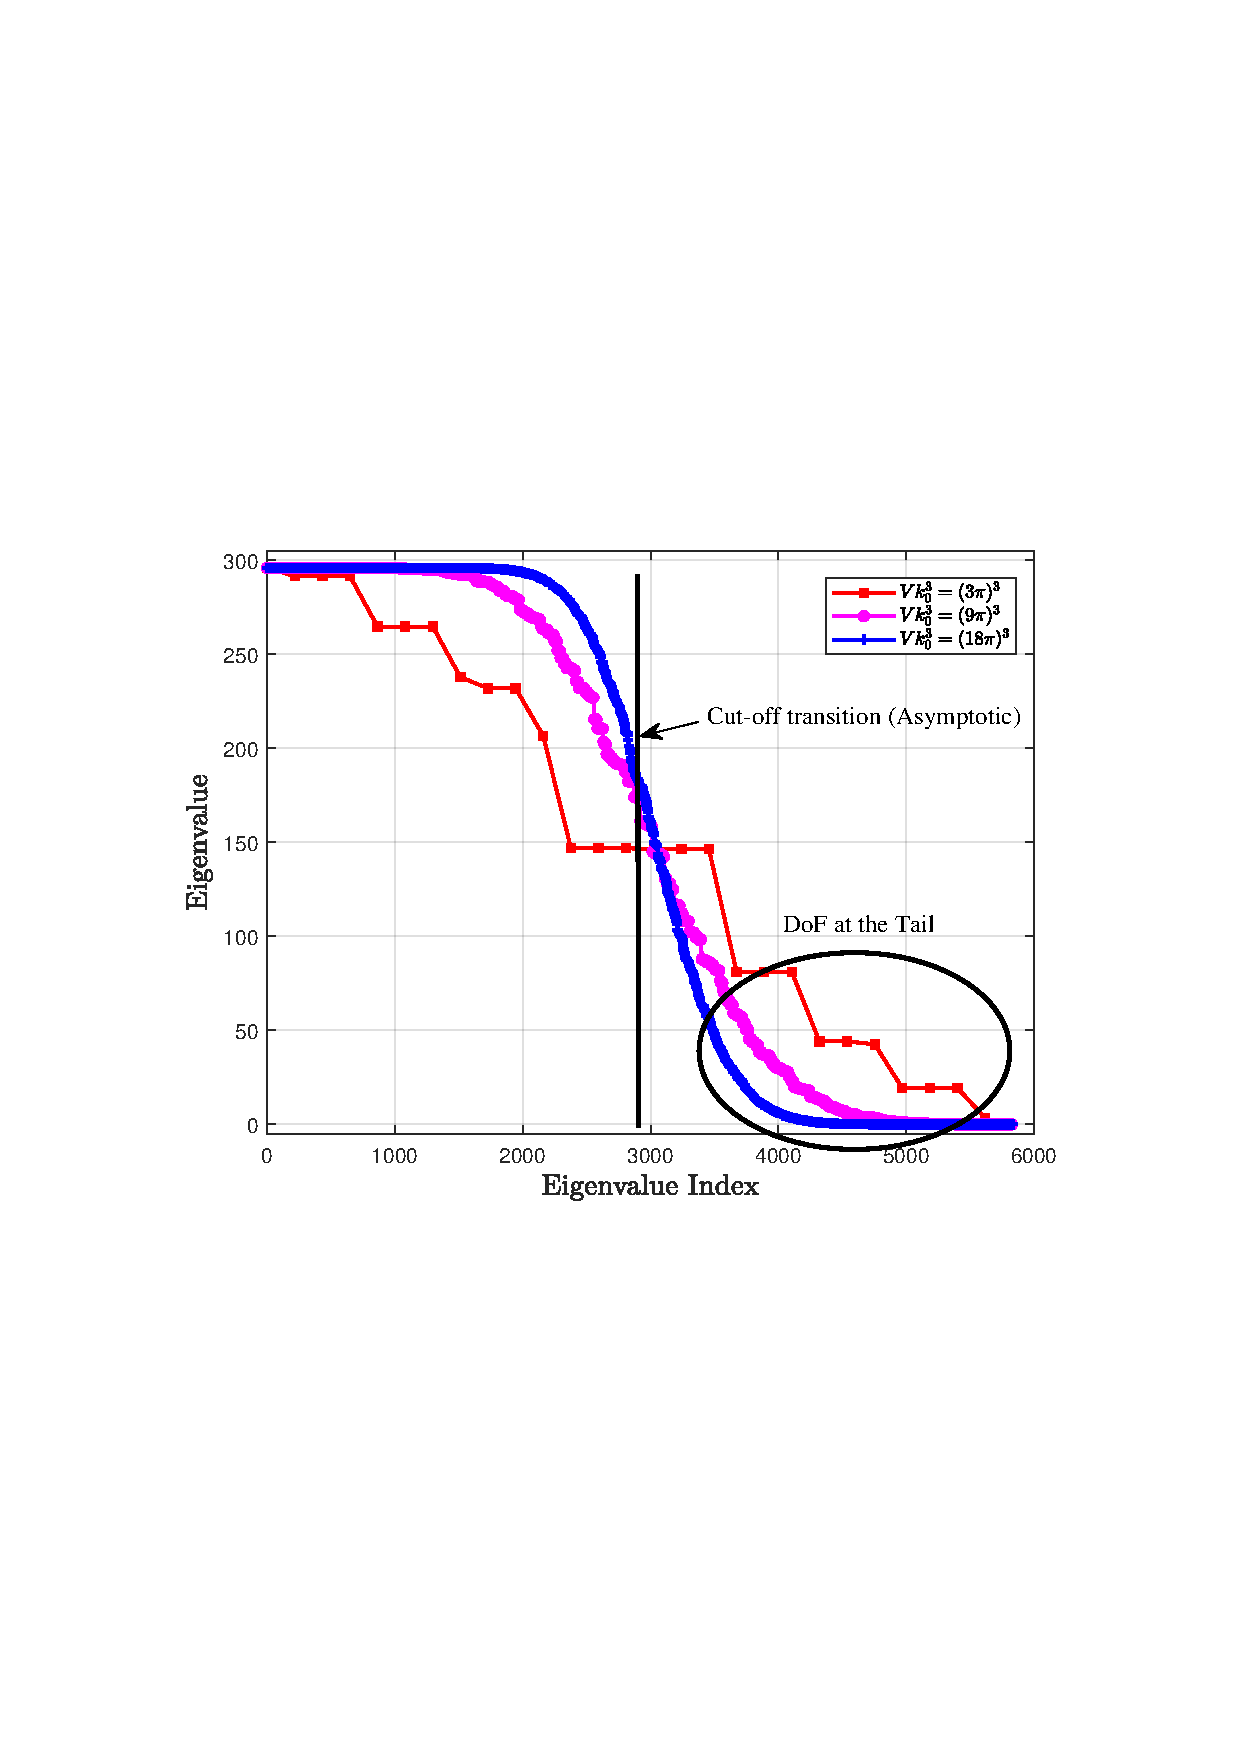
\includegraphics[width=0.7\textwidth]{figs/save_3d_different_Vk.pdf} 
   	\caption{\color{red} The eigenvalues of three-dimensional Slepian concentration problem when $V k_0^3$ increases.} 
   	\label{3d_Vk}
   \end{figure}
   {
   \color{red}
   \setcounter{remark}{5} 
   \begin{remark}
   	
   	(relationship between asymptotic and non-asymptotic DoF) In the above parts, we have discussed the models and schemes to analyze and solve the concentration problem for non-asymptotic DoF. Although it is hard to quantitatively discuss the exact value of non-asymptotic DoF, which relies on numerical calculations and the error bound $\epsilon$ as in {\bf Definition} 1, here we propose a conjecture whose generality remains unproven. More precisely, the non-asymptotic DoF with small $\epsilon$, although being obviously smaller than the asymptotic case that involves larger spatial and wavenumber constraint regions, will exceed the asymptotic case when both of them are averaged over the sizes of the spatial and wavenumber constraint regions. The reason is that observations confined to a finite region inherently exploit the structural characteristics of the field, which effectively convey partial information from outside the region. One observation of this phenomenon in the one-dimensional time-frequency case has been shown in Fig. 2, in which the dotted line (Cut-off transition) refers to the average DoF of asymptotic case. It can be observed that for finite $\Omega T$, the line has a tail at the right side of the Cut-off transition line, which is more obvious for smaller $\Omega T$. This tail means extra DoF above the average DoF when considering a small $\epsilon$. For the three-dimensional scenario in the space-wavenumber domain we also provide a numerical case in Fig. 3, which comes from the integral equation with kernel function (30). It can be observed that the same phenomenon also exists in the three-dimensional scenario, when considering average DoF over the sizes of the spatial and wavenumber constraint regions, the non-asymptotic case will exceed the asymptotic case. We have also found a similar phenomenon when considering mutual information with a finite observation window in the time domain [46].
   	
   	
   \end{remark}
   
   }
\end{framed}

{\color{blue}
	{\bf References:}
	
	[11] T. Gong, L. Wei, C. Huang, Z. Yang, J. He, M. Debbah, and C. Yuen, “Holographic MIMO communications with arbitrary surface
	placements: Near-field LoS channel model and capacity limit,” {\it IEEE J. Sel. Areas Commun.}, vol. 42, no. 6, pp. 1549–1566, Jun.
	2024.
	
	[12] L. Wei, C. Huang, G. C. Alexandropoulos, Z. Yang, J. Yang, E. Wei, Z. Zhang, M. Debbah, and C. Yuen, “Tri-polarized holographic
	MIMO surfaces for near-field communications: Channel modeling and precoding design,” {\it IEEE Trans. Wireless Commun.}, vol. 22,
	no. 12, pp. 8828–8842, Dec. 2023.
	
	[13] A. Pizzo, A. Lozano, S. Rangan, and T. L. Marzetta, “Wide-aperture MIMO via reflection off a smooth surface,” {\it IEEE Trans.
	Wireless Commun.}, vol. 22, no. 8, pp. 5229–5239, Aug. 2023.
	
	[30] D. Slepian and H. O. Pollak, “Prolate spheroidal wave functions, Fourier analysis and uncertainty—I,” {\it Bell System Technical
	Journal}, vol. 40, no. 1, pp. 43–63, Jan. 1961.
	
	[31] D. J. Thomson, “Spectrum estimation and harmonic analysis,” {\it Proc. IEEE}, vol. 70, no. 9, pp. 1055–1096, 2005.
	
	[32] T. M. Cover, Elements of information theory. John Wiley \& Sons, 1999.
	
	[33] H. Xiao, V. Rokhlin, and N. Yarvin, “Prolate spheroidalwavefunctions, quadrature and interpolation,” {\it Inverse problems}, vol. 17,
	no. 4, p. 805, 2001.
	
	[34] F. Furrer, M. Berta, M. Tomamichel, V. B. Scholz, and M. Christandl, “Position-momentum uncertainty relations in the presence
	of quantum memory,” {\it Journal of Mathematical Physics}, vol. 55, no. 12, 2014.
	
	[35] D. Slepian, “Prolate spheroidal wave functions, Fourier analysis and uncertainty—IV: extensions to many dimensions; generalized
	prolate spheroidal functions,” {\it Bell System Technical Journal}, vol. 43, no. 6, pp. 3009–3057, 1964.
	
	[36] F. J. Simons, F. Dahlen, and M. A. Wieczorek, “Spatiospectral concentration on a sphere,” {\it SIAM review}, vol. 48, no. 3, pp. 504–536,
	2006.
	
	[37] A. P. Bates, Z. Khalid, and R. A. Kennedy, “Slepian spatial-spectral concentration problem on the sphere: Analytical formulation
	for limited colatitude–longitude spatial region,” {\it IEEE Trans. Signal Process.}, vol. 65, no. 6, pp. 1527–1537, Mar. 2017.
	
	[38] G. Beylkin, C. Kurcz, and L. Monz´on, “Grids and transforms for band-limited functions in a disk,” {\it Inverse Problems}, vol. 23,
	no. 5, p. 2059, 2007.
	
	[39] F. J. Simons and D. V. Wang, “Spatiospectral concentration in the Cartesian plane,” {\it GEM-International Journal on Geomathematics},
	vol. 2, no. 1, pp. 1–36, 2011.
	
	[40] Y. Shkolnisky, “Prolate spheroidal wave functions on a disc—integration and approximation of two-dimensional bandlimited
	functions,” {\it Applied and Computational Harmonic Analysis}, vol. 22, no. 2, pp. 235–256, 2007.
	
	[41] J. Zhang, H. Li, L.-L. Wang, and Z. Zhang, “Ball prolate spheroidal wave functions in arbitrary dimensions,” {\it Applied and
	Computational Harmonic Analysis}, vol. 48, no. 2, pp. 539–569, 2020.
	
	[44] J. Reade, “Eigen-values of Lipschitz kernels,” in Mathematical Proceedings of the Cambridge Philosophical Society, vol. 93, no. 1.
	{\it Cambridge University Press}, 1983, pp. 135–140.
	
	
	[45] M. Belkin, “Approximation beats concentration? An approximation view on inference with smooth radial kernels,” {\it in Conference
	On Learning Theory. PMLR}, 2018, pp. 1348–1361.
	
	[46] J. Zhu, Z. Zhang, Z. Wan, and L. Dai, “On finite-time mutual information,” {\it in Proc. 2022 IEEE International Symposium on
	Information Theory (ISIT)}, 2022, pp. 2910–2915.
}

\textbf{Reviewer 2:}
6. On p8, “When n → $\infty$, F2(k) → $\delta$(k - k0)”,  the Dirac delta function is not well-defined. Does using a different representation for the delta function for F2(k) change the DoF?


{\color{blue}{\textbf{Authors: } 
Thanks for the reviewer's valuable comment. We have added more rigorous definitions about explanations about the delta function. We have also added explanations about why the DoF will not be changed when choosing a different representation for the delta function, which is guaranteed by the properties of the approximate identities [43].


The detailed revisions are shown as follows:
}}

\begin{framed}
	{\bf Section III. C}
	
	\setcounter{equation}{36}

The eigenvalues comes from the following integral equation
\begin{equation}
	\lambda_i f_i({\bf x}) = \int_{\mathcal{R}}D({\bf x},{\bf x}')f_i({\bf x}'){\rm d}^3{\bf x}'.
	\label{eigenfunction_3d}
\end{equation}
Here we set $\{F_{2,n}(k)\}_{n=1}^{+\infty} = \frac{1}{2h}\left( 1-\frac{|k-k_0|}{2h} \right), |k-k_0|\leqslant 2h$, $h = \frac{1}{2^n}$ to be a set of functions that make $F({\bf k})$ focus on a sphere surface in the wavenumber domain. When $n \rightarrow \infty$, $F_2(k) \rightarrow \delta(k-k_0)$. {\color{red} In a more rigorous description, we have $\underset{n \rightarrow +\infty}{\rm lim}{\int_{\mathbb{R}} F_2(k)f(k) } = f(k_0)$ for arbitrary smooth and compactly supported function $f(k) \in C_c^{\infty}({\mathbb R})$. It is worth noting that we use the function series $\{F_{2,n}(k)\}_{n=1}^{+\infty}$ due to two reasons. Firstly, we can establish the connection between the case where the support in the wavenumber domain has a continuous extent in $k$ (finite n), and the case localized only at the point $k_0$ ($n \rightarrow \infty$). Secondly, we can avoid directly using delta functions since they are not genuine functions but generalized functions, which possess some properties that can not be achieved by real-valued functions. Using a series of well-defined integrable functions, known as approximate identities, to approach the delta function is a common way used in existing literature [42]. From the above discussions, we can also observe that the functions $\{F_{2,n}(k)\}_{n=1}^{+\infty}$ can not be arbitrarily chosen. They should satisfy the power constraint $\int F_2(k) {\rm d}k = 1$ and describe a unit point mass at $k = k_0$ when $n \rightarrow \infty$ (or can be equivalently described as "support set shrinks to 0 when $n \rightarrow \infty$")
	from the limitation perspective
	[43]. 
	Then they all have the property $\underset{n \rightarrow +\infty}{\rm lim}{\int_{\mathbb{R}} F_2(k)f(k) } = f(k_0)$. There are infinite choices for such function series, but they have the same limitation as the delta function [43] and will lead to the same DoF.} 
\end{framed}
 
 {\color{blue}
 	{\bf References:}
 	
 	[42] R. S. Strichartz, A guide to distribution theory and Fourier transforms. World Scientific Publishing Company, 2003.
 	
 	[43] N. Wheeler, “Simplified production of Dirac delta function identities,” {\it Reed College}, 1997.
 }
 
 \textbf{Reviewer 2:}
7. What is the reason for introducing an approximation error $\epsilon$ in the definition of both functional and channel DoFs? For example, in the MIMO channel, the DoF is deterministic without any error terms. But why do the DoFs here have an error term?

 
 
 {\color{blue}{\textbf{Authors: } 
 Thanks for the reviewer's valuable question. The reason for introducing an approximation error $\epsilon$ is that we are considering continuous electromagnetic fields instead of discrete signals. In traditional discrete models we are using  discrete matrices which have finite ranks. However, for continuous electromagnetic fields, we are tackling Hilbert spaces with infinite dimensions. Now there is a contradiction between the theoretical model and practical schemes. In practical communication tasks, using an infinite number of base functions, which corresponds to infinite electromagnetic modes, is impossible and often unnecessary. The reason is that only a few base functions contribute a lot to the field reconstruction, while the remained base functions can be discarded with small loss of precision. The above observation motivates us to use the error $\epsilon$ to filter out unnecessary basis and obtain the number of basis we need, which is the DoF defined in the paper.
 		
 		
 According to the reviewer's comment, we have added more explanations about the reason for introducing $\epsilon$. The detailed revisions are shown as follows:
 }}
 
 \begin{framed}
 	{\bf Section II.B}
 	
 	{\color{red}
 	\quad As is shown in (\ref{eqn_dispersion_relation}), there are some physical restrictions that the electromagnetic fields should obey in wireless communication systems. These restrictions relate to time, frequency, space, and wavenumber domain. All possible electromagnetic fields considering these restrictions span a Hilbert space whose dimension is the number of basis needed to express an arbitrary field in the space. 
 	
 	\quad Note that, unlike a discrete matrix, the dimension of a continuous Hilbert space may be infinite. However, in practical communication tasks, using an infinite number of base functions, which corresponds to infinite electromagnetic modes, is impossible and often unnecessary. The reason is that only a few base functions contribute a lot to the field reconstruction, while the remained base functions can be discarded with small loss of precision. We will give a mathematical definition of the DoF based on the above discussion and verify its rationale in the following sections of the paper. 
 	}
 	\end{framed}

{\color{blue}{\textbf{Authors: } 
Many thanks again for your valuable time and efforts to review this paper. 
\\
\\
Sincerely, \\
{\it The Authors }
}}

\clearpage 

%%%%%%%%%%%%%%%%%%%%%%%%%%%%%%%%%%%%%%%%%%%%%%%%%%%%%%%%%%%%%%%%%%%%%%%%%%%%%%%%%%%%%
%%%%%%%%%%%%%%%%%%%%%%%%%%%%%%%%%%%%%%%%%%%%%%%%%%%%%%%%%%%%%%%%%%%%%%%%%%%%%%%%%%%%%
%%%%%%%%%%%%%%%%%%%%%%%%%%%%%%%%%%%%%%%%%%%%%%%%%%%%%%%%%%%%%%%%%%%%%%%%%%%%%%%%%%%%%
%%%%%%%%%%%%%%%%%%%%%%%%%%%%%%%%%%%%%%%%%%%%%%%%%%%%%%%%%%%%%%%%%%%%%%%%%%%%%%%%%%%%%


\begin{center}
    {\Large\bf Response to Reviewer 3's Comments}
\end{center}

\textbf{Reviewer 3:}
This paper presents some significant results of DoF in EIT. The extension of Slepian concentration theory to 3D and 4D domains under electromagnetic constraints is a significant theoretical contribution. This paper is well-structured and technically sound. This topic is interesting. My main comments are as follows.

{\color{blue}{\textbf{Authors: } 
We appreciate the reviewer's concise summary of the key points of this paper and the positive evaluations on our work. We have tried our best to address these issues in the revised paper according to the reviewer's concerns. Our responses are provided in a point-to-point manner as below. 
}}

\textbf{Reviewer 3:}
1. (Introduction) At the end of Page 3, you said “We use the theoretical analyzing tools from Slepian concentration problem and extend it to three-dimensional space domain and four-dimensional space-time domain under electromagnetic constraints”. More related works on Slepian concentration problem should be introduced. The challenges of such extension should be explained.

{\color{blue}{\textbf{Authors: } 
Thanks to the reviewer's valuable comment. We have added a new subsection as {\bf Section III.A} to explain the related works on Slepian concentration problem. These works involve different shapes of concentration regions and different dimensions of the related domains about the Slepian concentration problem, which mainly focus on mathematical analysis and numerical calculation schemes. Compared to these existing mathematical works, in this paper, we formulate the Slepian concentration problem in the three-dimensional space-wavenumber domain and the four-dimensional domain which also includes time-frequency. Our models are formulated based on physical constraints like the dispersion relation, from which we derive analytical forms of the kernel function $D({\bf x},{\bf x}')$. Then the eigenvalues which determine the DoF can be solved using the kernel function. How to integrate physical constraints with the concentration problem is the main challenge in the extension parts in the paper. In particular, in the case of single-frequency points, which is the focus of many recent papers, the subsequent analysis will show that the asymptotic conclusions completely lose their validity. 

The detailed revisions are shown in the following box:}}

\begin{framed}
	{\bf Section III}
	
	{\bf {\color{red} A. A brief introduction of the existing works on Slepian concentration problem}}
	
	{\color{red}
		\quad The original work, accomplished by Slepian, analyzed the one-dimensional time-frequency concentration problem which has analytical solutions for the eigenvalues and eigenfunctions [30]. Based on these analytical solutions, the number of large eigenvalues and the behavior of the decay rate of small eigenvalues can be directly analyzed. The results about the one-dimensional Slepian concentration problem serve as powerful tools, which have been widely adopted in many areas, including spectrum estimation [31], capacity analysis [32], numerical integration [33], uncertainty relations [34], etc.
		
		\quad Slepian has also discussed the possible extension of the concentration problem to high dimensions with sphere-shaped concentration region [35], but provided no analytical solutions for the eigenvalues. Many researchers have followed his work, analyzing the Slepian concentration problem with different domain representations and concentration regions. Due to the high complexity of the high-dimensional structures, even for highly symmetric models, the existing works still focus on numerical calculation schemes instead of finding analytical solutions for the eigenvalue and eigenfunction solutions. 
		
		\quad For the domain representation, one approach is constraining one domain on a sphere and the other domain using degrees and orders of spherical harmonic functions. An early work considering both asymptotic results and numerical calculations in non-asymptotic scenarios has been discussed in [36]. Further works added colatitude–longitude spatial region constraints on the sphere and provided numerical calculation schemes for the eigen-problem [37]. Since our DoF analysis is with the physical constraints in space-wavenumber domains, the constraints based on spherical harmonic functions do not well fit our needs. 
		
		\quad Another approach is directly considering two domains that are the Fourier transform or the inverse Fourier transform of each other. By directly performing sampling on the constraint regions, [38] considered the two-dimensional Slepian concentration problem with a disc-shaped constraint region in one domain and a rectangle-shaped region in the other domain. In a similar form, [39] considered disc-shaped constraint regions in both two domains. 
		The fast-converging numerical calculation scheme for evaluating the two-dimensional Slepian concentration problem was analyzed in [40], which considered disc-shaped constraints in two domains that are Fourier transform or inverse Fourier transform of each other. 
		Its further extension to higher dimensional balls was shown in [41], which also considered numerical schemes and had no analytical solutions. Moreover, these two papers considered an ideal case when the concentration regions in the two domains are both $n$-dimensional balls, while our concentration region in the space domain may not always have spherical symmetry. 
		
		\quad Compared to these existing mathematical works, in this paper, we will formulate the Slepian concentration problem in the three-dimensional space-wavenumber domain and the four-dimensional domain which also includes time-frequency. We will obtain the concentration region in the wavenumber domain based on physical constraints like the dispersion relation. How to integrate physical constraints with the concentration problem is the main challenge and the focus of the following parts in this section. In particular, in the case of single-frequency points, which is the focus of many recent papers [11]-[13], the subsequent analysis will show that the asymptotic conclusions completely lose their validity. Compared to spherical regions, we mainly focus on a cuboid-shaped spatial concentration region that fits transceivers in reality better, which will break the spherical symmetry and make performing theoretical analysis even harder.   
		
		\quad In all, we can find that providing analytical solutions for the eigenvalues and eigenfunctions when considering the Slepian concentration problem in high dimensions is very difficult. Therefore, obtaining numerical solutions after deriving the integral equations, which is not the best but is a practically feasible route, is chosen in our paper. Besides numerical simulations, we also provide some quantitative and qualitative analyses and discussions of the properties of the eigenvalues based on the derived kernel functions, which will be shown in the following parts.
	}

\end{framed}

{\color{blue}
	{\bf References:}
	
	[11] T. Gong, L. Wei, C. Huang, Z. Yang, J. He, M. Debbah, and C. Yuen, “Holographic MIMO communications with arbitrary surface
	placements: Near-field LoS channel model and capacity limit,” {\it IEEE J. Sel. Areas Commun.}, vol. 42, no. 6, pp. 1549–1566, Jun.
	2024.
	
	[12] L. Wei, C. Huang, G. C. Alexandropoulos, Z. Yang, J. Yang, E. Wei, Z. Zhang, M. Debbah, and C. Yuen, “Tri-polarized holographic
	MIMO surfaces for near-field communications: Channel modeling and precoding design,” {\it IEEE Trans. Wireless Commun.}, vol. 22,
	no. 12, pp. 8828–8842, Dec. 2023.
	
	[13] A. Pizzo, A. Lozano, S. Rangan, and T. L. Marzetta, “Wide-aperture MIMO via reflection off a smooth surface,” {\it IEEE Trans.
		Wireless Commun.}, vol. 22, no. 8, pp. 5229–5239, Aug. 2023.
	
	[30] D. Slepian and H. O. Pollak, “Prolate spheroidal wave functions, Fourier analysis and uncertainty—I,” {\it Bell System Technical
		Journal}, vol. 40, no. 1, pp. 43–63, Jan. 1961.
	
	[31] D. J. Thomson, “Spectrum estimation and harmonic analysis,” {\it Proc. IEEE}, vol. 70, no. 9, pp. 1055–1096, 2005.
	
	[32] T. M. Cover, Elements of information theory. John Wiley \& Sons, 1999.
	
	[33] H. Xiao, V. Rokhlin, and N. Yarvin, “Prolate spheroidalwavefunctions, quadrature and interpolation,” {\it Inverse problems}, vol. 17,
	no. 4, p. 805, 2001.
	
	[34] F. Furrer, M. Berta, M. Tomamichel, V. B. Scholz, and M. Christandl, “Position-momentum uncertainty relations in the presence
	of quantum memory,” {\it Journal of Mathematical Physics}, vol. 55, no. 12, 2014.
	
	[35] D. Slepian, “Prolate spheroidal wave functions, Fourier analysis and uncertainty—IV: extensions to many dimensions; generalized
	prolate spheroidal functions,” {\it Bell System Technical Journal}, vol. 43, no. 6, pp. 3009–3057, 1964.
	
	[36] F. J. Simons, F. Dahlen, and M. A. Wieczorek, “Spatiospectral concentration on a sphere,” {\it SIAM review}, vol. 48, no. 3, pp. 504–536,
	2006.
	
	[37] A. P. Bates, Z. Khalid, and R. A. Kennedy, “Slepian spatial-spectral concentration problem on the sphere: Analytical formulation
	for limited colatitude–longitude spatial region,” {\it IEEE Trans. Signal Process.}, vol. 65, no. 6, pp. 1527–1537, Mar. 2017.
	
	[38] G. Beylkin, C. Kurcz, and L. Monz´on, “Grids and transforms for band-limited functions in a disk,” {\it Inverse Problems}, vol. 23,
	no. 5, p. 2059, 2007.
	
	[39] F. J. Simons and D. V. Wang, “Spatiospectral concentration in the Cartesian plane,” {\it GEM-International Journal on Geomathematics},
	vol. 2, no. 1, pp. 1–36, 2011.
	
	[40] Y. Shkolnisky, “Prolate spheroidal wave functions on a disc—integration and approximation of two-dimensional bandlimited
	functions,” {\it Applied and Computational Harmonic Analysis}, vol. 22, no. 2, pp. 235–256, 2007.
	
	[41] J. Zhang, H. Li, L.-L. Wang, and Z. Zhang, “Ball prolate spheroidal wave functions in arbitrary dimensions,” {\it Applied and
		Computational Harmonic Analysis}, vol. 48, no. 2, pp. 539–569, 2020.
}

\textbf{Reviewer 3:} 2. (Introduction) The work [15] is based on the conclusions of Slepian concentration problem. What is the difference between your work and [15]?

{\color{blue}{\textbf{Authors: } 
Thanks to the reviewer's valuable question. The model used in [15] is limited to one-dimensional receivers, which is a simplification of real-world receivers with more complex structures in two-dimensional or three-dimensional space domains. Then [15] directly uses the conclusions of one-dimensional Slepian concentration problem to analyze the DoF. In this paper we formulate the Slepian concentration problem in the three-dimensional space-wavenumber domain and the four-dimensional domain which also includes time-frequency. We obtain the concentration region in the wavenumber domain based on physical constraints like the dispersion relation. Our work can be viewed as an extension of [15] by considering 1) more complex and realistic structures of the transceivers in the space domain; 2) the relationship between space-wavenumber domain and time-frequency domain.

The detailed revisions are shown in the following box:

}}

\begin{framed}
	{\bf Section I}

   \quad Therefore, there is a fundamental question in EIT that how many DoFs can be provided by a wireless communication system constrained by electromagnetism? Moreover, how can we utilize these DoFs to transfer information? For the analysis of DoFs in EIT, one approach is considering bandwidth in the wavenumber domain.  The bandwidth above is called spatial bandwidth in [14], which is similar to the widely-used bandwidth in time-frequency domain [20]. Identical to the time sampling scheme determined by classical bandwidth in the frequency domain, the bandwidth in wavenumber domain determines the sampling scheme in the space domain, which corresponds to the spatial DoF of the electromagnetic field. The spatial bandwidth of scattered fields was rigorously derived in [14]. It was shown that for a time-harmonic model with scatterers bounded in a sphere, the spatial bandwidth of the electromagnetic fields on an infinitely long observation line is linear with the frequency and the radius of the sphere. {\color{red} From the spatial bandwidth, the DoF obtained on a one-dimensional observation line is analyzed in [15] based on the conclusions of the Slepian concentration problem and prolate spheroidal wave functions. The model used in this work is limited to one-dimensional receivers, which is a simplification of real-world receivers with more complex structures in two-dimensional or three-dimensional space domains.} For arbitrary received fields on a two-dimensional surface, half-wavelength sampling scheme in the spatial domain was obtained in [21] when evanescent waves were discarded, which provided insightful results about the bound of DoF from direct spatial sampling. However, the spatial sampling requires infinite observation regions in the spatial domain, which is not consistent with practical wireless communication systems with finite spatial regions. {\color{red} Moreover, while the real-world communication systems simultaneously involve mutually-coupled time and space domains, the time domain is omitted in the above works.}

\end{framed}

{\color{blue}
	{\bf References:}
	
	[14] O. Bucci and G. Franceschetti, “On the spatial bandwidth of scattered fields,” {\it IEEE Trans. Antennas Propag.}, vol. 35, no. 12, pp.
	1445–1455, Dec. 1987.
	
	[15] O. M. Bucci and G. Franceschetti, “On the degrees of freedom of scattered fields,” {\it IEEE Trans. Antennas Propag.}, vol. 37, no. 7,
	pp. 918–926, Jul. 1989.
	
	[20] D. Slepian, “On bandwidth,” {\it Proc. of the IEEE}, vol. 64, no. 3, pp. 292–300, Mar. 1976.
	
	[21] C. A. Balanis, Antenna theory: Analysis and design. John wiley \& sons, 2015.
	
}


\textbf{Reviewer 3:} 3. (Sec II-A) How to obtain the eigenvalues in Fig. 1?

{\color{blue}{\textbf{Authors: } 
Thanks to the reviewer's valuable question. We obtain the eigenvalues in Fig. 1 (Now Fig. 2 in the revised paper) by numerically solving the integral equation (18). Some quadrature rules can be used to replace $\int$ by $\sum$, which change the eigen-problem of a continuous operator to the eigen-problem of a discrete matrix. The convergence of using the quadrature rules can be guaranteed by Nyström’s method [50]. Here we use midpoint rule to discretize the operator.

According to the reviewer's comments, we have explained how we obtain the eigenvalues in the figure, shown in the following box:
}}

\begin{framed}
	{\bf Section III. B}

    We show in Fig. 2 that when $\Omega T \rightarrow \infty$, the decay line of eigenvalues will have a cut-off transition. {\color{red} Here we use numerical schemes to solve the integral equation (18) to obtain Fig. 2. Specifically, we substitute $\int$ by $\sum$ in (18) and solve the corresponding eigen-problem of matrix generated by $D(t,t')$. Since in the one-dimensional case the solutions for (18) has analytical forms [30], directly using these solutions can also obtain the same result.}
\end{framed}

{\color{blue}
	{\bf References:}
	
	[30] D. Slepian and H. O. Pollak, “Prolate spheroidal wave functions, Fourier analysis and uncertainty—I,” {\it Bell System Technical
	Journal}, vol. 40, no. 1, pp. 43–63, Jan. 1961.
	
	[50] A. Spence, “On the convergence of the Nystr¨om method for the integral equation eigenvalue problem,” {\it Numerische Mathematik},
	vol. 25, no. 1, pp. 57–66, 1975.
	
	
}

\textbf{Reviewer 3:} 4. (Sec II-A) Should $\lambda$ in (3) be $\lambda_i$?

{\color{blue}{\textbf{Authors: } 
Thanks the reviewer for pointing out this problem. We have revised the problem in the paper (now in (18) and (25)).

 Detailed revisions are shown as:
}}

\begin{framed}
{\bf Section III.B}

\setcounter{equation}{17}

Then for a bandlimited signal $G(\omega) = \int_{-T}^{+T}g(t)e^{-{\rm j}\omega t}{\rm d}t$, the optimally concentrated signal is taken to be the one that maximizes $\lambda = \frac{\int_{-\Omega}^{\Omega}|G(\omega)|^2{\rm d}\omega}{\int_{-\infty}^{\infty}|G(\omega)|^2{\rm d}\omega}$, which leads to the following integral equation
\begin{equation}
	\begin{aligned}
		\int_{-T}^{T}D(t,t'){\color{red}g_i}(t'){\rm d}t' = {\color{red}\lambda_{i} g_i(t)},
	\end{aligned}
	\label{eqn_1d_t}
\end{equation}

\setcounter{equation}{24}

The integral equation corresponding to the two-dimensional eigenfunctions and eigenvalues is 
\begin{equation}
	\begin{aligned}
		\int_{\mathcal{R}}D({\bf x},{\bf x}'){\color{red}f_i({\bf x}')}{\rm d}^2{\bf x}' = {\color{red}\lambda_i f_i({\bf x})},
	\end{aligned}
	\label{eqn_2d_integral}
\end{equation}
    
\end{framed}

\textbf{Reviewer 3:}
5. (Sec II-B) What’s the definition of V in (14) and (16)?

{\color{blue}{\textbf{Authors: } 
Thanks the reviewer for pointing out this problem. The notation $V$ represents the volume of the $\mathcal{R}$, which is the concentration region in the space domain. We have added the definitions of $V$ in the revised paper.
The detailed revisions are shown below:

}}

\begin{framed}
{\bf Section III.C}

\setcounter{equation}{27}

{\color{red} We denote the concentration region in the space domain as $\mathcal{R}$, and the concentration region in the wavenumber domain as $\mathcal{K}$.} For the first case similar to what has been discussed in one-dimensional and two-dimensional examples, we have 
\begin{equation}
	\begin{aligned}
		f({\bf x})=(2\pi)^{-3}\int_{-\infty}^{+\infty}F({\bf k})e^{{\rm j}{\bf k}\cdot {\bf x}}{\rm d}^3{\bf k},
	\end{aligned}
\end{equation}
and
\begin{equation}
	\begin{aligned}
		F({\bf k}) = \int_{-\infty}^{+\infty}f({\bf x})e^{-{\rm j}{\bf k}\cdot {\bf x}}{\rm d}^3{\bf x}.
	\end{aligned}
\end{equation}
If the wavenumber domain constraint satisfies $k_x^2+k_y^2+k_z^2 \leqslant k_0^2$, we have 
\begin{equation}
	\begin{aligned}
		D({\bf x},{\bf x}') &= (2\pi)^{-3}\int_{\mathcal{K}} e^{{\rm j}{\bf k}\cdot({\bf x}-{\bf x}')}{\rm d}^3{\bf k} \\&= (2\pi)^{-3} \int_{0}^{k_0} \int_{{\Omega}=\{\hat{\bf k}: \left\| \hat{\bf k} \right\|=1\}} e^{{\rm j}k\hat{\bf k}\cdot({\bf x}-{\bf x}')}k^2{\rm d}^2S{\rm d}k
		\\& = (2\pi)^{-3} 4\pi \int_0^{k_0} \frac{\sin k \left\| {\bf x}-{\bf x}' \right\|}{k \left\| {\bf x}-{\bf x}' \right\|}k^2 {\rm d}k
		\\& = \frac{1}{2\pi^2} \left( \frac{\sin k\left\| {\bf x}-{\bf x}' \right\|}{\left\| {\bf x}-{\bf x}' \right\|^3}-\frac{k\cos k\left\| {\bf x}-{\bf x}' \right\|}{\left\| {\bf x}-{\bf x}' \right\|^2} \right) \Bigg|_0^{k_0}
		\\& = \frac{1}{2\pi^2} \left( \frac{\sin k_0\left\| {\bf x}-{\bf x}' \right\|}{\left\| {\bf x}-{\bf x}' \right\|^3}-\frac{k_0\cos k_0\left\| {\bf x}-{\bf x}' \right\|}{\left\| {\bf x}-{\bf x}' \right\|^2} \right).
	\end{aligned}
	\label{equ_ball}
\end{equation}
The asymptotic DoF is 
\begin{equation}
	\begin{aligned}
		N^{3D} = \sum_{i=1}^\infty \lambda_i = \int_{\mathcal{R}}D({\bf x},{\bf x}){\rm d}^3{\bf x} = \frac{V}{6\pi^2}k_0^3,
	\end{aligned}
\end{equation}
{\color{red} where $V$ is the volume of $\mathcal{R}$.}


\end{framed}

\textbf{Reviewer 3:}
6. (Sec II-B) The classic Slepian concentration result is extended to three-dimensional case with constraints on the wavenumber domain. It seems like the core is to derive the kernel function D. Then, the DoF problem can be transformed to an integral problem. Though it is challenging to obtain the main results in this part, more important analysis is lacking. When I read the introduction part, especially “the non-asymptotic case which does not require sufficiently large transceivers or sufficiently large frequency bandwidth has not been discussed yet. Since practical wireless communication systems suit non-asymptotic cases better than asymptotic cases, discussing the DoF under non-asymptotic cases is of importance”, what I expect is clear non-asymptotic expressions, and the relationship between non-asymptotic results and asymptotic DoF in order. Could you provide more analysis?

{\color{blue}{\textbf{Authors: } 
Thanks for the reviewer for pointing out this problem. We agree with the reviewer that discussing the non-asymptotic case is important. As is shown in {\bf Section III.A}, providing analytical solutions for the integral equations derived when considering Slepian concentration problems in three and four-dimensional domains is very hard and still not done by existing mathematical works. If the analytical solutions can be obtained, the DoF problem is perfectly answered. However, at this stage we have not obtained these solutions. 

Instead, to strengthen the theoretical parts in non-asymptotic cases, in the revised paper, we have added some new qualitative and quantitative discussions about the derived kernel functions, which show some insights about the DoF. These insights include the decay rate of the eigenvalues which determine the number of DoF, the difference when considering non-asymptotic DoF with wide band and single-frequency point scenarios, and the characteristics of the eigenfunctions which serve as the eigen-modes of the electromagnetic fields.

For the second problem about the relationship between non-asymptotic results and asymptotic DoF. We have a conjecture that the non-asymptotic DoF with small $\epsilon$, although being obviously smaller than the asymptotic case that involves larger spatial and wavenumber constraint regions, will exceed the asymptotic case when both of them are averaged over the sizes of the spatial and wavenumber constraint regions. The reason is that observations confined to a finite region inherently exploit the structural characteristics of the field, which effectively convey partial information from outside the region. 

The detailed revisions are shown in the following box:
}}

\begin{framed}
	{\bf Section III.C}

\setcounter{equation}{46}

{\color{red}
	
	\quad From {\bf Remark} 5 we have shown how the eigenvalues of the Slepian concentration problem influence the fDoF of the electromagnetic field. Now we will have some discussions about the properties of the eigenvalues, including the decay rate, the possible large values, and their relationship with the varying speed of the eigenfunctions, etc. These properties can also be observed in the numerical simulation part. 
	
	\quad We now focus on the kernel functions $D_1({\bf x},{\bf x}')=\frac{1}{2\pi^2} \left( \frac{\sin k_0\left\| {\bf x}-{\bf x}' \right\|}{\left\| {\bf x}-{\bf x}' \right\|^3}-\frac{k_0\cos k_0\left\| {\bf x}-{\bf x}' \right\|}{\left\| {\bf x}-{\bf x}' \right\|^2} \right)$ in (30) and $D_2({\bf x},{\bf x}') = \frac{1}{2\pi^2} \frac{k_0\sin k_0 \left\| {\bf x}-{\bf x}' \right\|}{\left\|  {\bf x}-{\bf x}' \right\|}$ in (42), as they represent two extreme cases with full band $(0,\omega_0]$ and single-frequency point $\omega_0$. First of all, we will discuss the decay rate of the eigenvalues of the integral operators with these two kernels. In [44], the eigenvalues obey the rule $\lambda_n  = o(n^{-k-1})$, where $k$ is the order of differentiability of the kernel function of the integral operator. Therefore, determining the differentiability (smoothness) helps to predict the long-term behavior of the eigenvalues.
	It is easy to observe that $D_1({\bf x},{\bf x}')$ and $D_2({\bf x},{\bf x}')$ are real analytic if we do not consider the point ${\bf x} = {\bf x}'$. Now we will examine if they are real analytic at ${\bf x} = {\bf x}'$. 
	Note that $D_1({\bf x},{\bf x}')$ and $D_2({\bf x},{\bf x}')$ are determined by $\left\|{\bf x}-{\bf x}'\right\|$. We only need to check the radial functions $E_1(r) = \frac{1}{2\pi^2} \left( \frac{\sin k_0 r}{r^3} - \frac{k_0 \cos k_0 r}{r^2} \right)$ and $E_2(r) = \frac{1}{2 \pi^2} \frac{k_0 \sin k_0 r}{r}$ at the origin $r = 0$. Utilizing Taylor's expansion, we have 
	\begin{equation}\begin{aligned}\sin(k_0r)&=k_0r-\frac{(k_0r)^3}{6}+\frac{(k_0r)^5}{120}+O(r^7),\\\cos(k_0r)&=1-\frac{(k_0r)^2}{2}+\frac{(k_0r)^4}{24}+O(r^6),\end{aligned}\end{equation}
	which means that the Taylor expansions of $E_1(r)$ and $E_2(r)$ only contain even powers of $r$ and ensures the real analyticity of $D_1$ and $D_2$. Then we know that these two kernels are smooth or infinitely differentiable. From {\bf Theorem 5} in [45], it was shown that the eigenvalues $\{\lambda_n\}$ of a smooth radial kernel defined in a $d$-dimensional space can be upper-bounded by $\lambda_n \leqslant C' e^{-C n^{1/d}}$ where $C$ and $C'$ are constants related to the kernel. Therefore, we can conclude that the eigenvalues of the integral operators with kernel $D_1$ and $D_2$ will decay to 0 with sub-exponential speed.   
	
	\quad Moreover, when checking the Fourier transforms of the kernel functions $D_1$ and $D_2$, it is easy to observe from their derivation procedure that $D_1$ has a broader basis on $k \in (0,k_0]$ while $D_2$ only on a single point. Then from a qualitative perspective, we know that $D_1$ and $D_2$ have the same spherical symmetry in the wavenumber domain. Their difference exists in the radius dimension. To be more specific,
	$D_1$ excites all possible modes that are below the frequency limit $w_0$, which tends to result in a series of similar large eigenvalues. On the contrary, $D_2$ only excites one mode at the frequency point $w_0$, which tends to result in one or only a few large eigenvalues. 
	
	\quad It is also worth noting that the integral operators mentioned above can be viewed as low-pass filters since they tend to keep the slow-varying components due to the smoothness of the kernels. Therefore, it is expected that when solving the concentration problem, the eigenfunctions that more slowly on the space domain will correspond to larger eigenvalues. According to {\bf Remark} 5, these eigenfunctions serve as good electromagnetic bases since they are more important when constructing required transmitted fields compared to other eigenfunctions, which will be verified in the simulation parts.
}

{
	\color{red}
	\setcounter{remark}{5} 
	\begin{remark}
		
		(relationship between asymptotic and non-asymptotic DoF) In the above parts, we have discussed the models and schemes to analyze and solve the concentration problem for non-asymptotic DoF. Although it is hard to quantitatively discuss the exact value of non-asymptotic DoF, which relies on numerical calculations and the error bound $\epsilon$ as in {\bf Definition} 1, here we propose a conjecture whose generality remains unproven. More precisely, the non-asymptotic DoF with small $\epsilon$, although being obviously smaller than the asymptotic case that involves larger spatial and wavenumber constraint regions, will exceed the asymptotic case when both of them are averaged over the sizes of the spatial and wavenumber constraint regions. The reason is that observations confined to a finite region inherently exploit the structural characteristics of the field, which effectively convey partial information from outside the region. One observation of this phenomenon in the one-dimensional time-frequency case has been shown in Fig. 2, in which the dotted line (Cut-off transition) refers to the average DoF of asymptotic case. It can be observed that for finite $\Omega T$, the line has a tail at the right side of the Cut-off transition line, which is more obvious for smaller $\Omega T$. This tail means extra DoF above the average DoF when considering a small $\epsilon$. For the three-dimensional scenario in the space-wavenumber domain we also provide a numerical case in Fig. 3, which comes from the integral equation with kernel function (30). It can be observed that the same phenomenon also exists in the three-dimensional scenario, when considering average DoF over the sizes of the spatial and wavenumber constraint regions, the non-asymptotic case will exceed the asymptotic case. We have also found a similar phenomenon when considering mutual information with a finite observation window in the time domain [46].
		
		
	\end{remark}
	
	   \setcounter{figure}{2}
	\begin{figure}[H]
		\centering 
		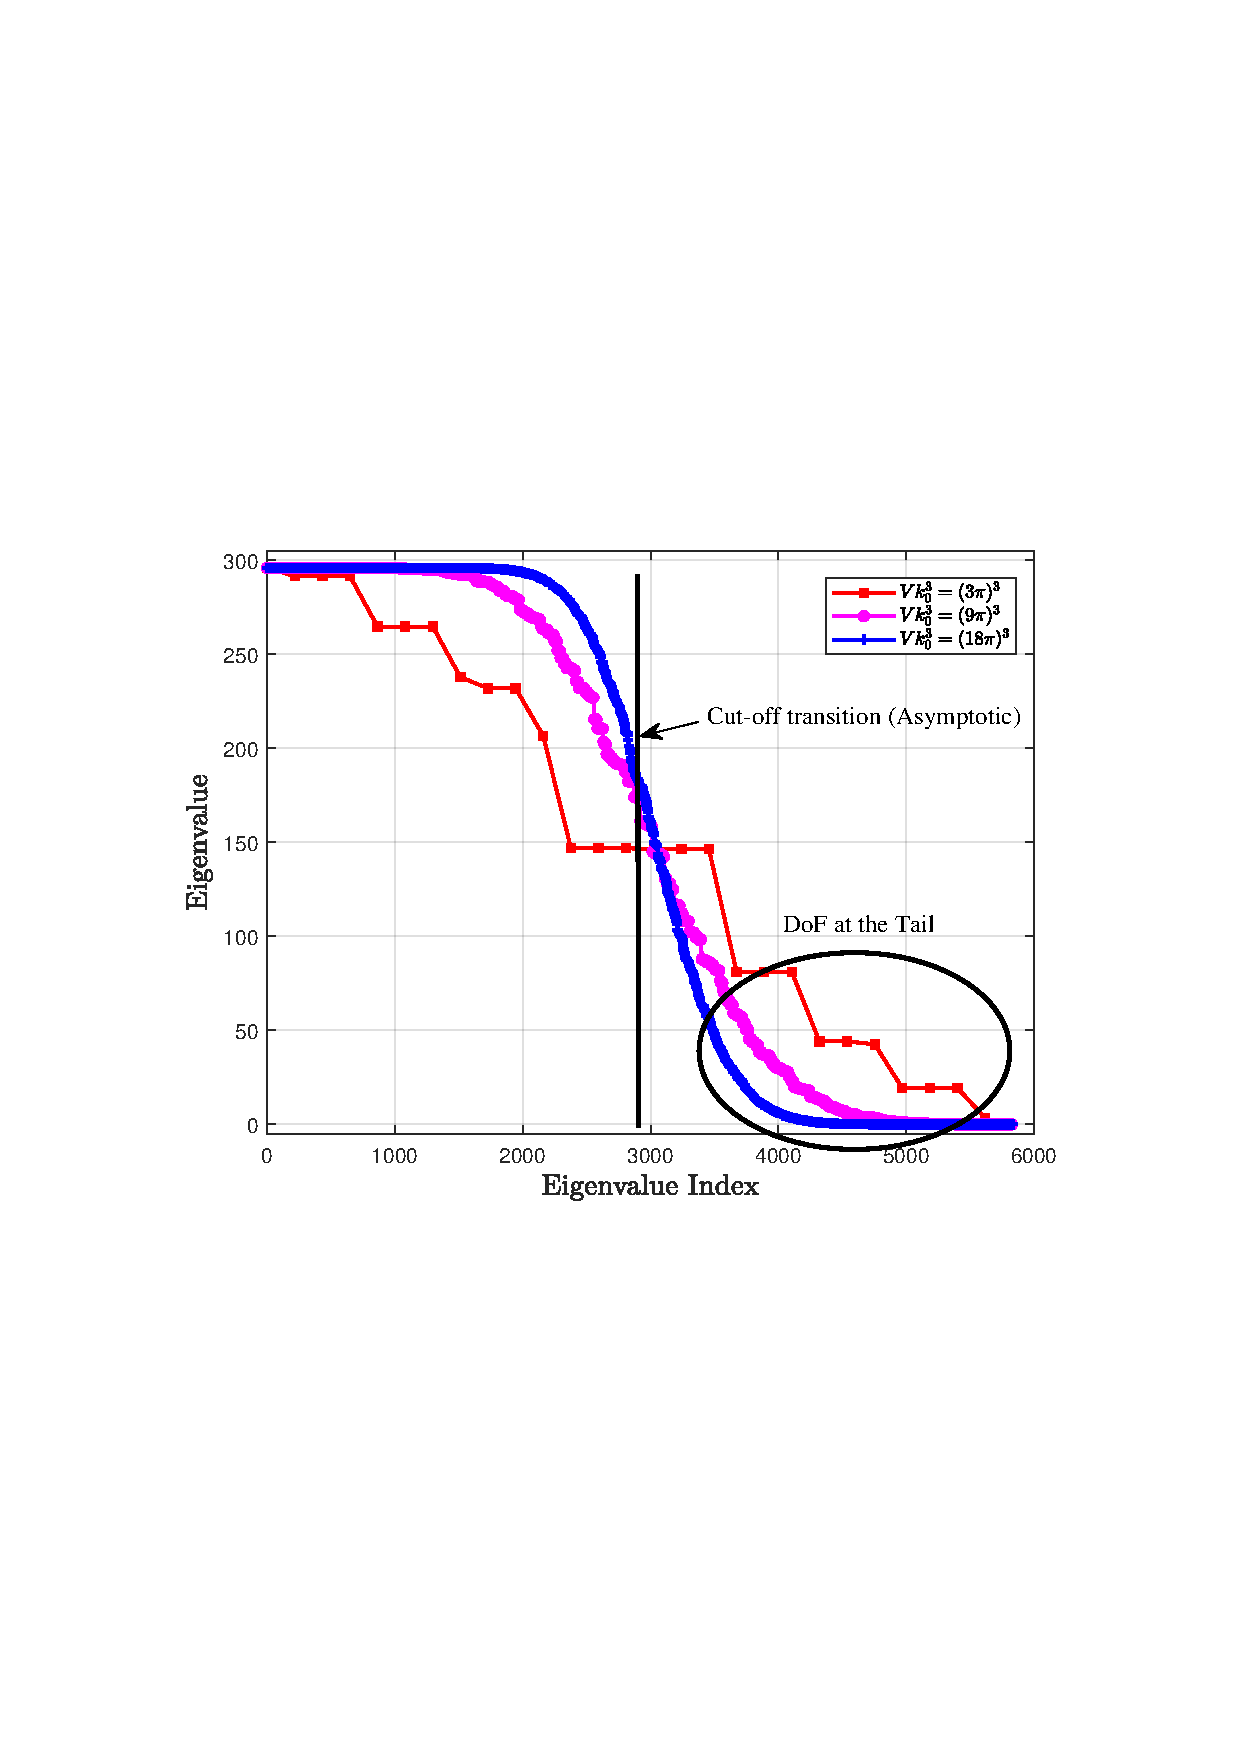
\includegraphics[width=0.7\textwidth]{figs/save_3d_different_Vk.pdf} 
		\caption{\color{red} The eigenvalues of three-dimensional Slepian concentration problem when $V k_0^3$ increases.} 
		\label{3d_Vk}
	\end{figure}
}
\end{framed}

{\color{blue}
	{\bf References:}
	
	[44] J. Reade, “Eigen-values of Lipschitz kernels,” in Mathematical Proceedings of the Cambridge Philosophical Society, vol. 93, no. 1.
	{\it Cambridge University Press}, 1983, pp. 135–140.
	
	
	[45] M. Belkin, “Approximation beats concentration? An approximation view on inference with smooth radial kernels,” {\it in Conference
		On Learning Theory. PMLR}, 2018, pp. 1348–1361.
	
	[46] J. Zhu, Z. Zhang, Z. Wan, and L. Dai, “On finite-time mutual information,” {\it in Proc. 2022 IEEE International Symposium on
		Information Theory (ISIT)}, 2022, pp. 2910–2915.
}

\textbf{Reviewer 3:}
7. (Sec II-C) Could you provide some discussions on the differences between 1-, 2-, 3-, and 4-dimention results?

{\color{blue}{\textbf{Authors: } 
Thanks for the reviewer's valuable problem. The one-dimensional case corresponds to the model with ideal transceivers on a line in the spatial domain. In the wavenumber domain, two of the three variables $k_x$, $k_y$, and $k_z$ are omitted. The constraint region in this case is the projection of the original constraint region in the three-dimensional domain to only one dimension of it. The two-dimensional case is similar to the one-dimensional case. It is easy to observe that some structural information is lost in such a projection. We have added a new figure (Fig. 5) in the paper to show the three different 3d structures of constraint regions in the wavenumber domain. These three structures will lead to different DoFs and sampling schemes in the spatial domain. However, when projecting them to the two-dimensional domain, all of them degenerate to the same disc, losing the information that exists in the third dimension. Therefore, we claim that analyzing the concentration problem in the three-dimensional space-wavenumber domain is better than lower dimensions, which preserves more information of the original electromagnetic field. 

For the 4-dimensional case, we further consider the time domain to extend the dimensions of the problem. By incorporating the time domain into the system model, it becomes possible to characterize the joint properties of electromagnetic waves across both space and time domains in a more unified manner. This enables the construction of time–space joint electromagnetic bases, which, in contrast to conventional designs that decouple space and time, may bring additional performance gains. The underlying reason lies in the dispersion relation from Maxwell's equations, which intrinsically couples the Fourier representation in the time domain with that in the space domain, thereby making the two domains inseparable in essence. It is interesting to find that the Minkowski spacetime interval $s^2 = c^2(t-t')^2 - \left\| {\bf x}-{\bf x}' \right\|^2$ exists in the four-dimensional integral kernel function (62), which reflects the inherent compatibility of Maxwell’s equations with the framework of special relativity [49]. Since it is the pole of the kernel function, it is associated with the eigenmodes of the electromagnetic field. When this term equals 0, we can get the light-cone relation $\left\| {\bf x}-{\bf x}' \right\|= c|t-t'|$, which reflects the causal structure of the field when transmitting.

We have added the discussions on the differences between 1-, 2-, 3-, and 4-dimention results as a new comment in {\bf Section III.D}. Detailed revisions in the paper are shown in the following box:
}}

\begin{framed}
	{\bf Section III.D}

{\color{red}
	\setcounter{remark}{7} 
	\begin{remark}
		(relationship and differences between cases with different dimensions) After introducing and analyzing all the concentration problems based on one-dimensional, two-dimensional, three-dimensional and four-dimensional cases, now we will discuss the relationship and differences between them. First of all, the one-dimensional case, although originally used in the time-frequency domain, can be used in the space-wavenumber domain considering only one dimension. In other words, this case corresponds to the model with ideal transceivers on a line in the spatial domain. In the wavenumber domain, two of the three variables $k_x$, $k_y$, and $k_z$ are omitted. The constraint region in this case is the projection of the original constraint region in the three-dimensional domain to only one dimension of it. The two-dimensional case is similar, which is not repeated here. It is easy to observe that some structural information is lost in such a projection. For example, we show the three different structures of constraint regions in the wavenumber domain that have been discussed in Section III.C in previous subsections. These three structures will lead to different DoFs and sampling schemes in the spatial domain. However, when projecting them to the two-dimensional domain as formulated in (\ref{eqn_2d_integral}), all of them degenerate to the same disc, losing the information that exists in the third dimension. Therefore, we claim that analyzing the concentration problem in the three-dimensional space-wavenumber domain is better than lower dimensions, which preserves more information of the original electromagnetic field. 
		
		Besides the three-dimensional space-time domain, we further consider the time domain to extend the dimensions of the problem to four. By incorporating the time domain into the system model, it becomes possible to characterize the joint properties of electromagnetic waves across both space and time domains in a more unified manner. This enables the construction of time–space joint electromagnetic bases, which, in contrast to conventional designs that decouple space and time, may bring additional performance gains. The underlying reason lies in the dispersion relation from Maxwell's equations, which intrinsically couples the Fourier representation in the time domain with that in the space domain, thereby making the two domains inseparable in essence. It is interesting to find that the Minkowski spacetime interval $s^2 = c^2(t-t')^2 - \left\| {\bf x}-{\bf x}' \right\|^2$ exists in the four-dimensional integral kernel function (62), which reflects the inherent compatibility of Maxwell’s equations with the framework of special relativity [49]. Since it is the pole of the kernel function, it is associated with the eigenmodes of the electromagnetic field. When this term equals 0, we can get the light-cone relation $\left\| {\bf x}-{\bf x}' \right\|= c|t-t'|$, which reflects the causal structure of the field when transmitting.
		
	\end{remark}
	
	\setcounter{figure}{4}
	\begin{figure}[H]
		\centering 
		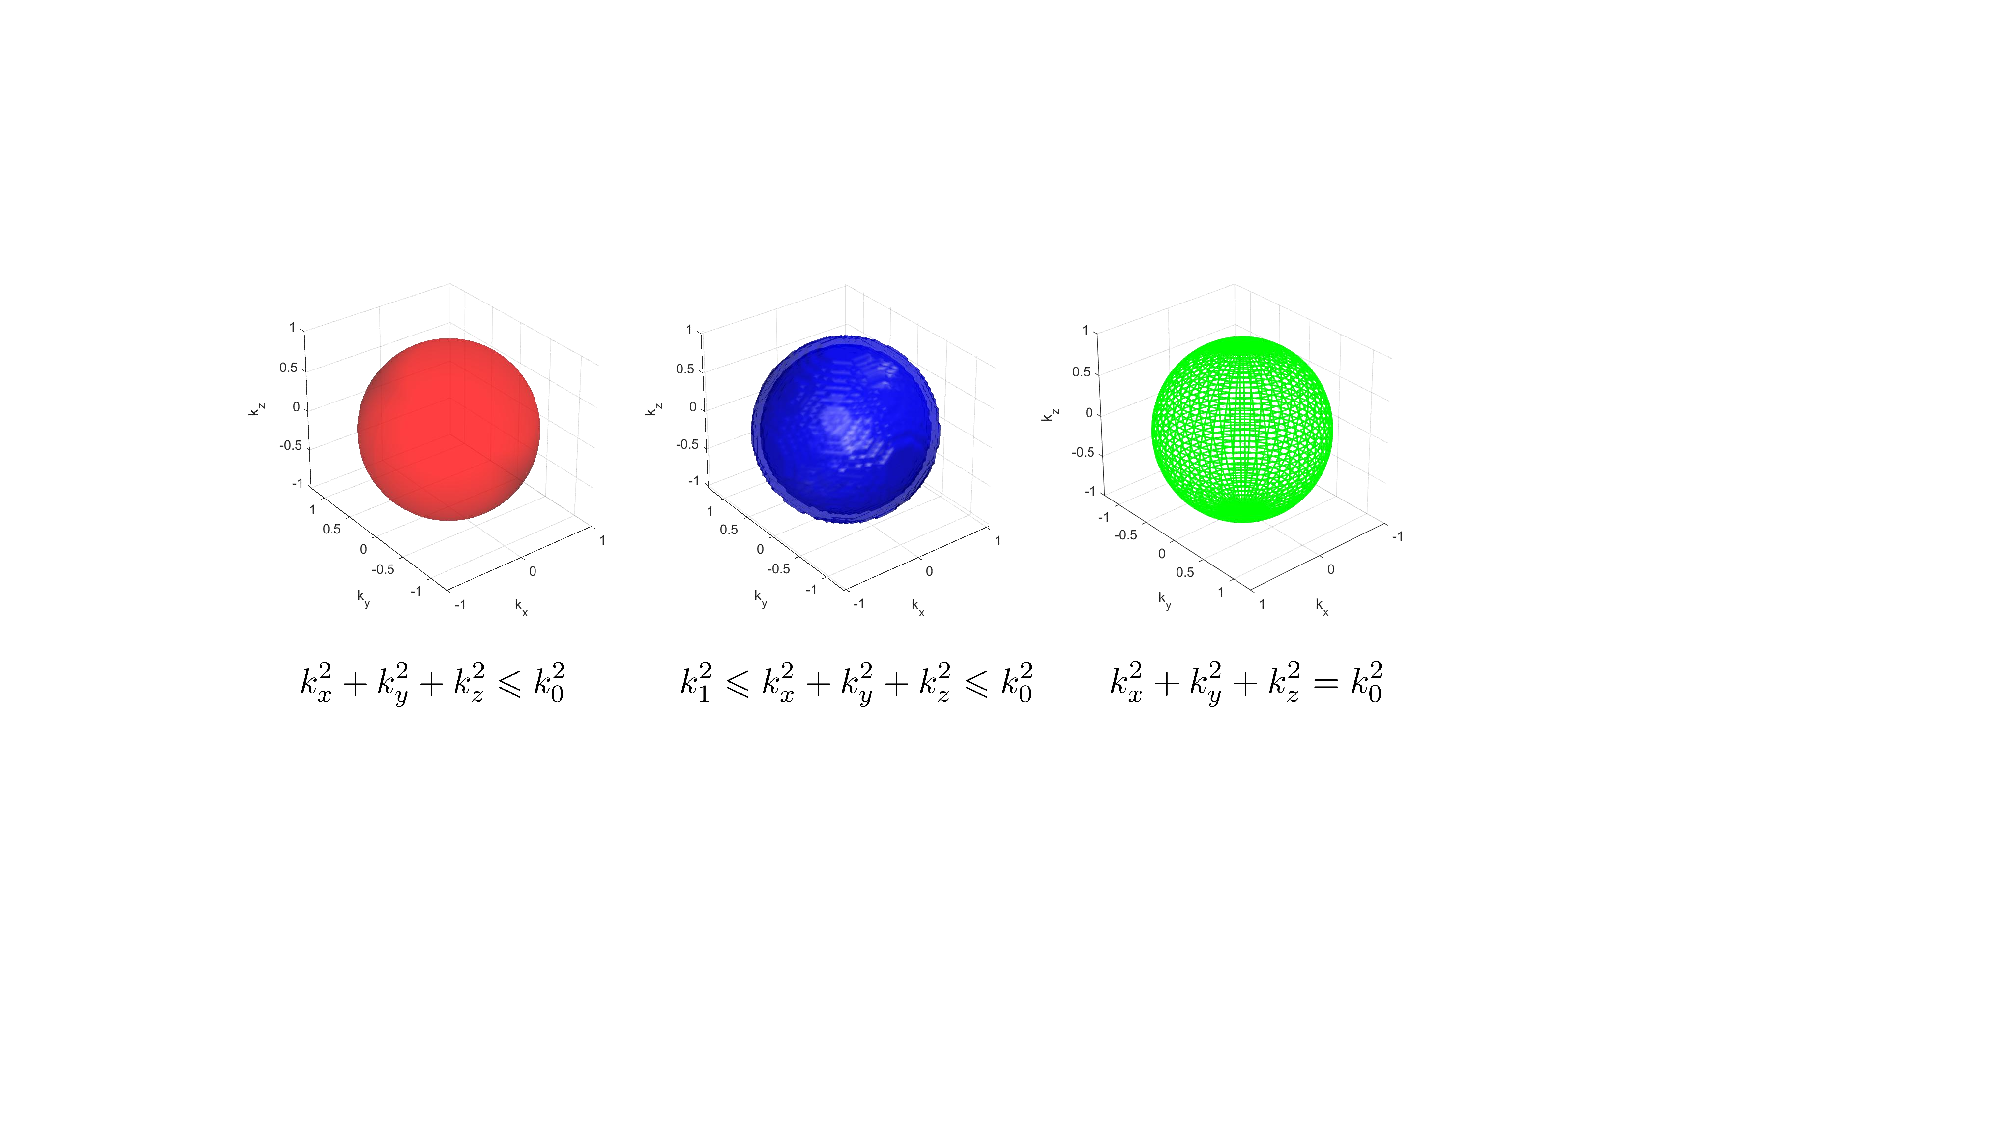
\includegraphics[width=0.7\textwidth]{figs/Three_d_comparison.pdf} 
		\caption{\color{red} Three different structures of constraint regions in wavenumber domain.} 
		\label{Three_d_comparison}
	\end{figure}
}
\end{framed}

{\color{blue}
	{\bf References:}
	
	[49] J. Schwinger, L. L. DeRaad Jr, K. Milton, and W.-y. Tsai, Classical electrodynamics. CRC Press, 2019.
}

\textbf{Reviewer 3:}
8. (Sec III) Could the cDoF lower-bounded by a term related to fDoF? This can make the analysis on fDoF more significant.

{\color{blue}{\textbf{Authors: } 
		Thanks for the reviewer's valuable comment. Whether we can obtain a lower-bound or not depends on the characteristics of the channel operator $P$. If we do not have extra information on $P$, it is difficult to find a new inequality that makes the cDoF lower-bounded by a term related to fDoF. To be more specific, we assume that each function in $\mathcal{H}_{\rm r}$ has a preimage in $\mathcal{H}_{\rm t}$ through the projection $P$. According to the definition of fDoF in $\mathcal{H}_{\rm r}$ we know that there exists a function $f\in \mathcal{H}_{\rm r}$ with modulus 1 that at least $n$ bases should be used to represent it with error $\epsilon_2$. Let $Pg = f$ and $\left\| g\right\| = a$, we know that the channel DoF with error $\epsilon_2/a$ should be no less than $fDoF_{\epsilon_2}(\mathcal{H}_r)$. From {\bf Lemma} 1 we know that $a \geqslant 1/\left\|  P \right\|$ but can not know the upperbound of $a$, which relies on $P$ and determines the lower bound of cDoF. If we denote the upperbound of $a$ by $a_0$, it is obvious that $cDoF_{a_0\epsilon_2}(\mathcal{H}_t,\mathcal{H}_r,P)\geqslant fDoF_{\epsilon_2}(\mathcal{H}_r)$.
		
		
		We have added a new remark in {\bf Section II.D} to clarify this problem. The detailed revisions are shown as follows:
		
	}}

\begin{framed}
	{\bf Section III.D}
	
	{\color{red}
		\setcounter{remark}{2} 
		\begin{remark}
In {\bf Theorem 2} we provide an upperbound of cDoF using fDoF. While a lowerbound will further strengthen the work, it highly relies on the characteristics of the channel operator $P$. Now we will show the reason. We assume that each function in $\mathcal{H}_{\rm r}$ has a preimage in $\mathcal{H}_{\rm t}$ through the projection $P$. According to the definition of fDoF in $\mathcal{H}_{\rm r}$ we know that there exists a function $f\in \mathcal{H}_{\rm r}$ with modulus 1 that at least $n$ bases should be used to represent it with error $\epsilon_2$. Let $Pg = f$ and $\left\| g\right\| = a$, we know that the channel DoF with error $\epsilon_2/a$ should be no less than $fDoF_{\epsilon_2}(\mathcal{H}_r)$. From {\bf Lemma} 1 we know that $a \geqslant 1/\left\|  P \right\|$ but can not know the upperbound of $a$, which relies on $P$ and determines the lower bound of cDoF. If we denote the upperbound of $a$ by $a_0$, it is obvious that $cDoF_{a_0\epsilon_2}(\mathcal{H}_t,\mathcal{H}_r,P)\geqslant fDoF_{\epsilon_2}(\mathcal{H}_r)$. 

\end{remark}
}

\end{framed}

\textbf{Reviewer 3:}
9. (Sec IV) It is interesting to obtain some results on the optimal antenna spacing. You mentioned that “It can be observed from Fig. 6 that by applying half-wavelength sampling on the two-dimensional array, nearly all eigenvalues are above zero, which means that half-wavelength sampling is necessary to utilize the DoF of the electromagnetic fields.” What is the theoretic support for the connection between antenna spacing and eigenvalues? Is the optimal antenna spacing related to fDoF or cDof?

{\color{blue}{\textbf{Authors: } 
		Thanks for the reviewer's valuable question. The connection between the antenna spacing and eigenvalues can be presented from two perspectives. The first perspective concerns the approximation process in numerical computation. The point at which the number of non-zero eigenvalues tends to stabilize, without further significant growth as the discretization order increases, indicates that the performance of the spatial sampling has become close to that of the continuous case. The second perspective concerns the limiting DoF obtained through this approximation. When considering antenna spacing, the model corresponds to using delta functions as basis functions to represent the band-limited fields, instead of the eigenfunctions solved from the concentration problem. From a qualitative standpoint, the required discretization order, which relates to the optimal antenna spacing, is comparable to the number of non-zero eigenvalues. These two perspectives are the supports when we use eigenvalues to show the optimal or near-optimal antenna spacing in the simulation part. 
		
		As the reviewer says, the optimal antenna spacing is related to $cDoF$ and $fDoF$, depending on whether we are designing the transceivers for a specific channel condition or for general channel conditions.
		For a specific channel condition, the optimal antenna spacing relates to $cDoF$, while for all possible kinds of channel conditions, the optimal antenna spacing relates to $fDoF$. 
		
		To better explain these points in the paper, we have added some explanations about the physical meaning of the numerical calculation schemes at the beginning of {\bf Section IV}. Then we add a new comment in {\bf Section IV} clarifying the connection between the antenna spacing and eigenvalues. Detailed revisions are shown in the following box:
	}}

\begin{framed}
	{\bf Section IV}
	
	\setcounter{equation}{62}
	
{\color{red}
	\quad It is worth noting that all the theoretical derivations above are based on the electromagnetic fields constrained in continuous regions. The distribution of eigenvalues characterizes the number of eigenfunctions required to approximate any desired continuous electromagnetic field using the obtained eigenfunction basis, which requires solving the eigen-problem of an integral operator $T := \phi({\bf x}) \rightarrow \int_{\mathcal{R}} K({\bf x},{\bf x}')\phi({\bf x}') {\rm d}^3 {\bf x}'$ or $T := \phi({\bf x},t) \rightarrow \int_{\mathcal{T}}\int_{\mathcal{R}} K({\bf x},t,{\bf x}',t')\phi({\bf x}',t') {\rm d}^3 {\bf x}'{\rm d} {t}'$ with kernel function $K$ solved in {\bf Section} III.C and III.D. Take the four-dimensional case as an example, the eigen-problem is formulated as the following integral equation
	\begin{equation}
		\lambda_i \phi_i({\bf x},t) = T \phi_i({\bf x},t).
	\end{equation}
	In the simulation part, we consider numerical discretization methods, which can be viewed as using a model that divides the continuous region into several spatially discretized regions. The discretization order $n$ corresponds to the number of antennas and time-observation points used in practical engineering problems, where each antenna provides one observation of the electromagnetic field within a given discretized spatial region. The eigenvalues and eigenvectors of the discretized matrix are then used as counterparts to the eigenvalues and eigenfunctions of the continuous operator in the theoretical analysis. To be more specific, we have a discretized matrix ${\bf K}$ with ${\bf K}_{i,j} = w_j K({\bf x}_i,t_i,{\bf x}_j,t_j)$, where ${w}_{i=1}^n$, ${\bf x}_{i=1}^n$, and $t_{i=1}^n$ are chosen by numerical integral quadrature rules on the regions $\mathcal{R}$ and $\mathcal{T}$. Then, the eigenproblem is formulated as the integral equation
	\begin{equation}
		\lambda'_i {\bf v} = {\bf K} {\bf v}.
	\end{equation}
	As the discretization order increases, Nyström’s method ensures that the matrix eigenvalues converge to those of the continuous operator, which can be found in {\bf Theorem 7} in [50]. 
}
	
	{\color{red}
		\setcounter{remark}{10} 
		\begin{remark}
			(Connection between antenna spacing and eigenvalues) Here, we discuss the relationship between the antenna spacing and eigenvalues from two perspectives. The first perspective concerns the approximation process in numerical computation. The point at which the number of non-zero eigenvalues tends to stabilize, without further significant growth as the discretization order increases, indicates that the performance of the spatial sampling has become close to that of the continuous case. The second perspective concerns the limiting DoF obtained through this approximation. When considering antenna spacing, the model corresponds to using delta functions as basis functions to represent the band-limited fields, instead of the eigenfunctions solved from the concentration problem. From a qualitative standpoint, the required discretization order, which relates to the optimal antenna spacing, is comparable to the number of non-zero eigenvalues. For a specific channel condition, the optimal antenna spacing relates to $cDoF$, while for all possible kinds of channel conditions, the optimal antenna spacing relates to $fDoF$. 
			However, since the basis using delta functions is not the optimal one provided by the concentration problem, a slightly larger number of basis functions may be needed to achieve the same approximation performance. 
			
		\end{remark}
	}
	
\end{framed}

{\color{blue}
	{\bf References:}
	
	[50] A. Spence, “On the convergence of the Nystr¨om method for the integral equation eigenvalue problem,” {\it Numerische Mathematik},
	vol. 25, no. 1, pp. 57–66, 1975.
	
}


{\color{blue}{\textbf{Authors: } 
Many thanks again for your valuable time and efforts to review this paper. 

Sincerely, \\
{\it The Authors }
}}


\clearpage 


\end{document}
